% Created 2019-05-09 Thu 17:29
% Intended LaTeX compiler: pdflatex
\documentclass[12pt, a4paper]{article}
\usepackage[utf8]{inputenc}
\usepackage[T1]{fontenc}
\usepackage{graphicx}
\usepackage{grffile}
\usepackage{longtable}
\usepackage{wrapfig}
\usepackage{rotating}
\usepackage[normalem]{ulem}
\usepackage{amsmath}
\usepackage{textcomp}
\usepackage{amssymb}
\usepackage{capt-of}
\usepackage{hyperref}
\usepackage[style=authoryear,natbib]{biblatex}
\setlength\bibitemsep{\baselineskip}
\addbibresource{/Users/guilhermesalome/Dropbox/references.bib}
\usepackage[T1]{fontenc}
\usepackage{lmodern}
\usepackage{amsmath}
\usepackage{mathtools}
\usepackage{multirow}
\usepackage{booktabs}
\usepackage{bbm}
\newcommand\numberthis{\addtocounter{equation}{1}\tag{\theequation}}
\newcommand{\E}[1]{\mathbb{E}{\left[#1\right]}}
\newcommand{\EQ}[1]{\mathbb{E}_t^{\mathbb{Q}}{\left[#1\right]}}
\newcommand{\EP}[1]{\mathbb{E}_t^{\mathbb{P}}{\left[#1\right]}}
\newcommand{\e}[1]{\text{e}^{#1}}
\newcommand{\abs}[1]{\left\vert{#1}\right\vert}
\newcommand{\dis}{\overset{d}{\sim}}
\newcommand{\Var}[1]{\mathrm{Var}\left(#1\right)}
\newcommand{\Corr}[1]{\mathrm{Corr}\left(#1\right)}
\newcommand{\Normal}[1]{\mathcal{N}\left(0, #1\right)}
\newcommand{\Max}[1]{\text{max}\left\{#1\right\}}
\newcommand{\Set}[1]{\left\{#1\right\}}
\renewcommand{\ln}[1]{\text{ln}\left(#1\right)}
\DeclareMathOperator*{\argmin}{\arg\!\min}
\DeclareMathOperator*{\argmax}{\arg\!\max}
\DeclarePairedDelimiter\ceil{\lceil}{\rceil}
\DeclarePairedDelimiter\floor{\lfloor}{\rfloor}
\newcommand{\Poisson}[1]{\text{Poisson}\left(#1\right)}
\newcommand{\Uniform}[1]{\text{Unif}#1}
\newcommand{\Cov}[1]{\mathrm{Cov}\left(#1\right)}
\newtheorem{problem}{Problem}
\usepackage[hang,small,bf]{caption}
\usepackage[margin=1in]{geometry}
\usepackage{mathtools}
\usepackage{xcolor}
\usepackage{resizegather}
\usepackage{multirow}
\definecolor{darkgreen}{rgb}{0.1, 0.6, 0.1}
\usepackage{fancyhdr}
\pagestyle{fancy}
\fancypagestyle{plain}{}
\fancyhf{}
\rfoot{Page \thepage}
\usepackage{ifthen}
\rhead{\ifthenelse{\value{page}=1}{Guilherme Salom\'{e}}{Summer \the\year}}
\lhead{\ifthenelse{\value{page}=1}{Econ890-01 Matlab}{Econ890-01 Matlab}}
\usepackage[numbered,framed]{matlab-prettifier}
\usepackage{listings}
\date{}
\title{Matlab Basics}
\hypersetup{
 pdfauthor={Guilherme Salomé},
 pdftitle={Matlab Basics},
 pdfkeywords={},
 pdfsubject={},
 pdfcreator={Emacs 26.1 (Org mode 9.2.1)},
 pdflang={English}}
\begin{document}

\maketitle
\section{The Matlab Integrated Development Environment}
\label{sec:orgad76206}
When Matlab is first opened you are presented with an integrated development environment (IDE), which is depicted in Figure \ref{fig:orgc7f2154} below.

\begin{figure}[!ht]
\centering
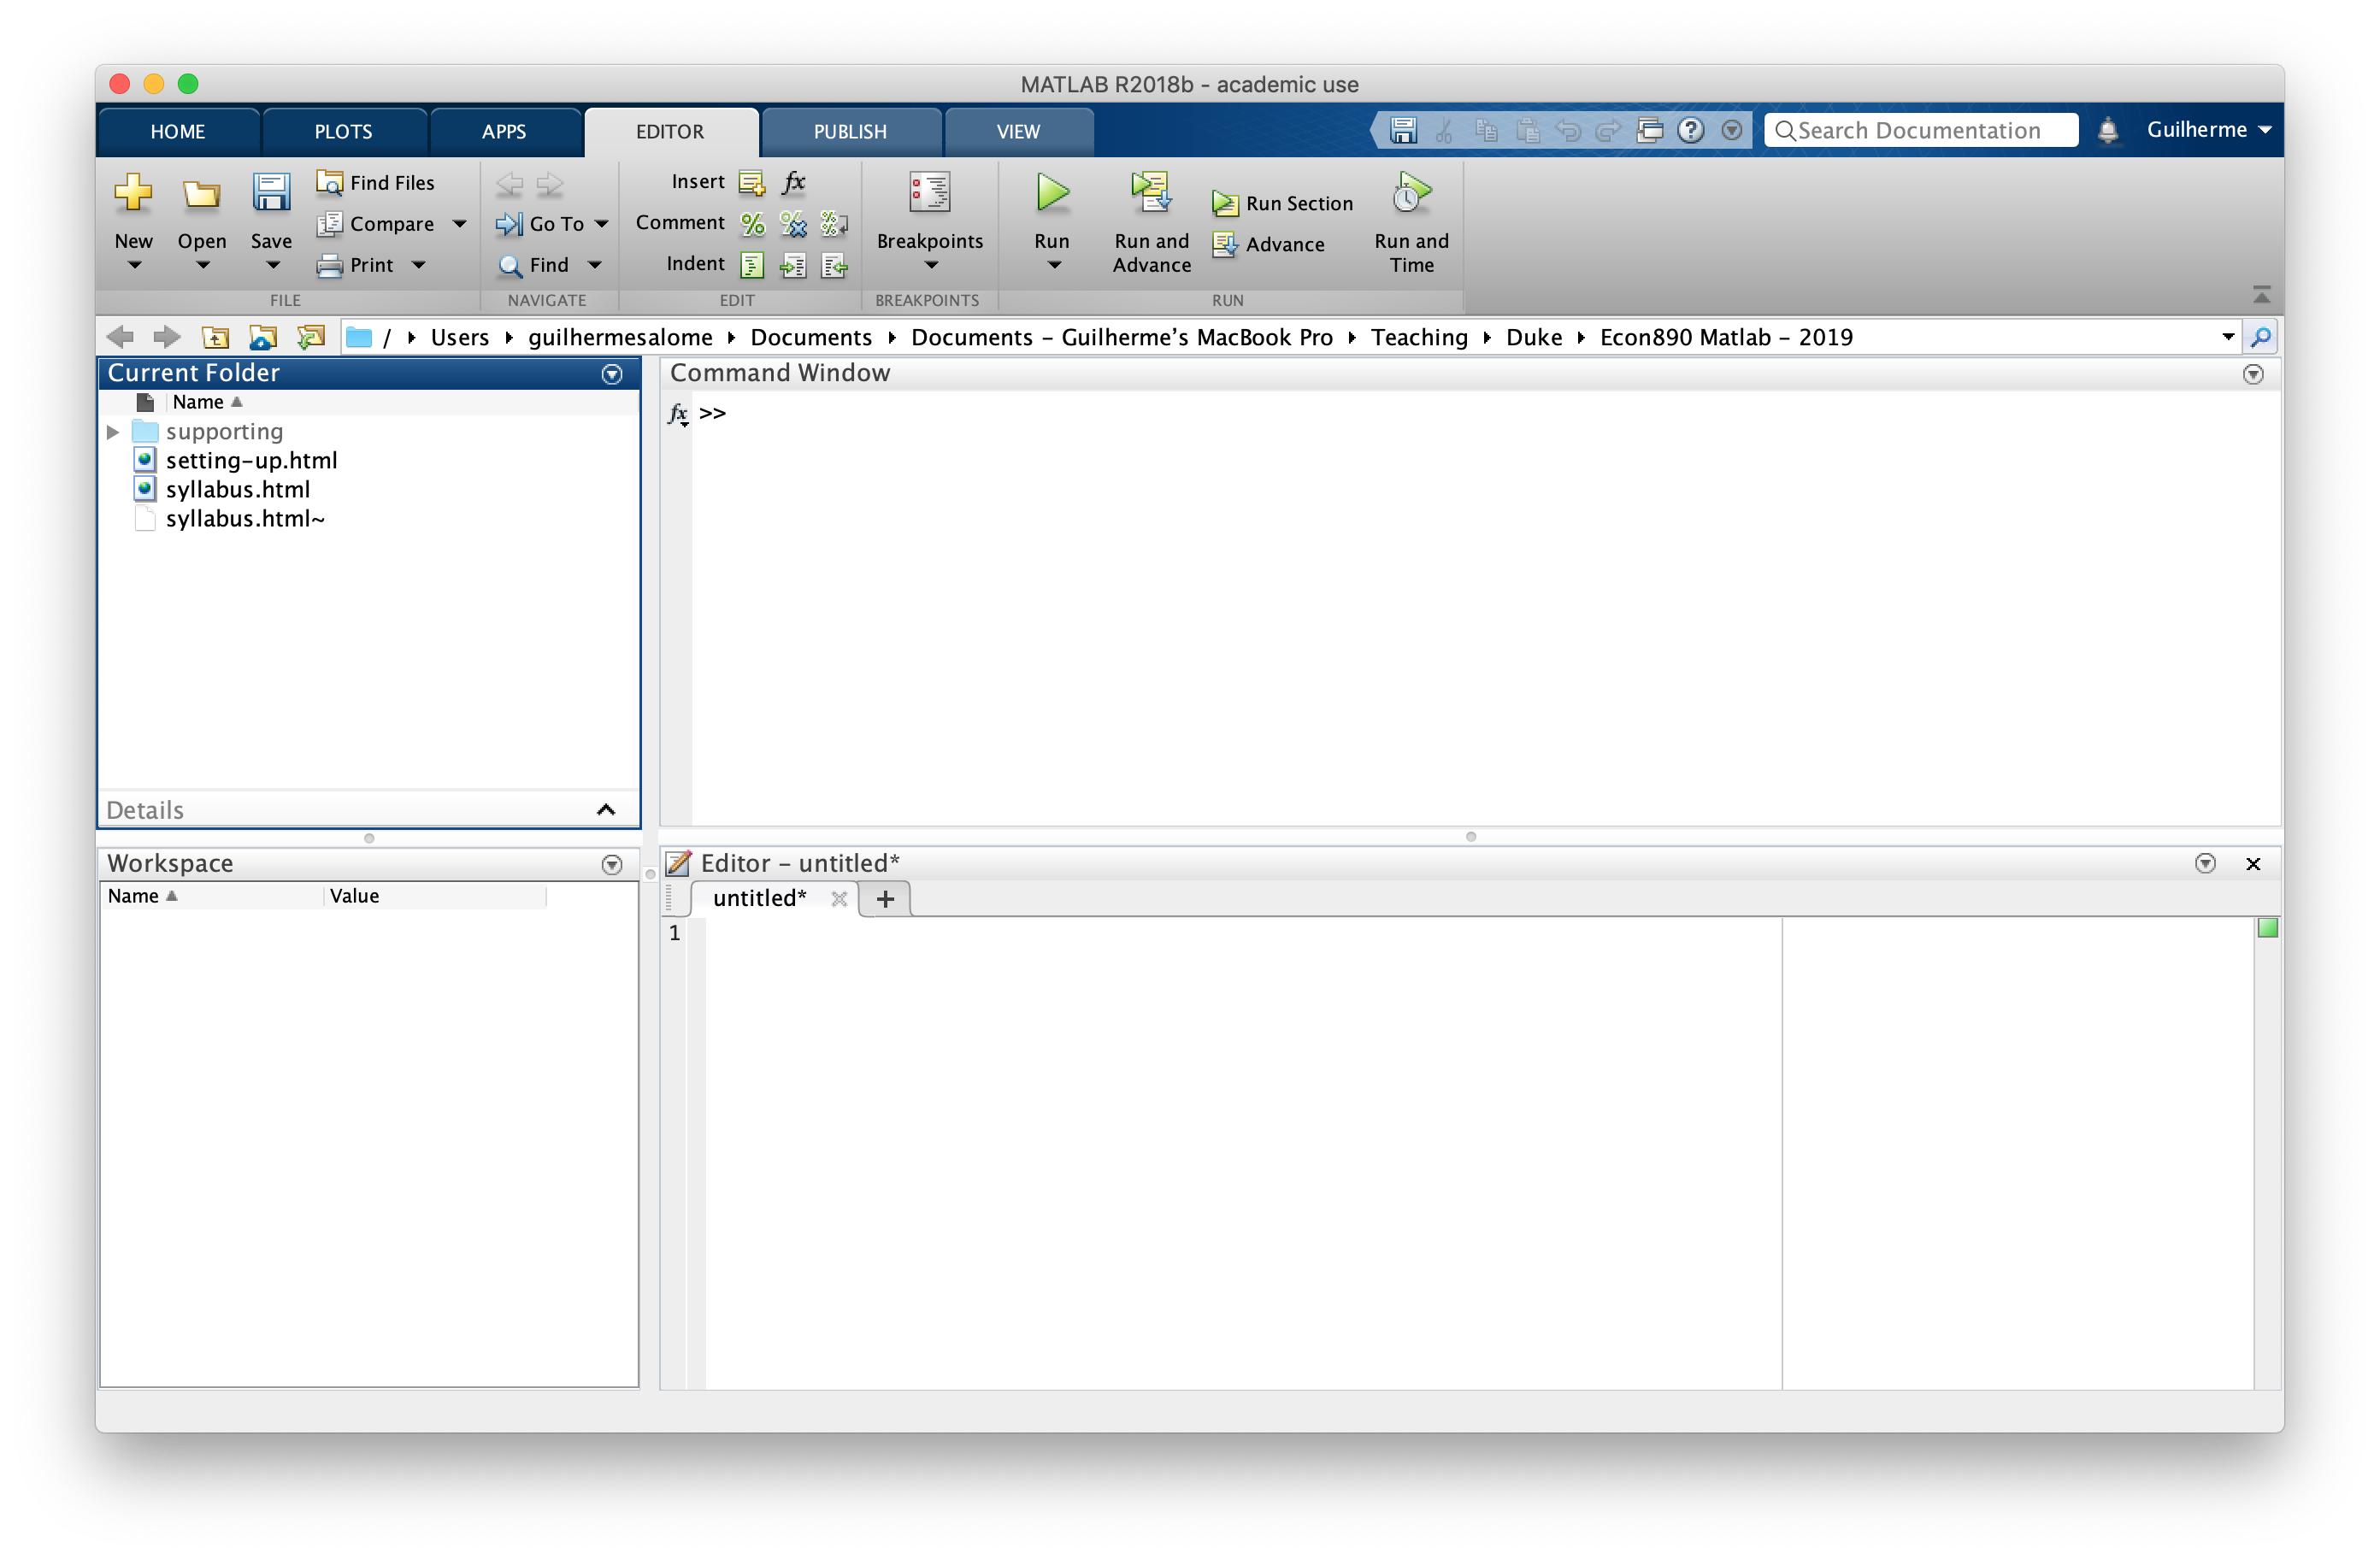
\includegraphics[width=.9\linewidth]{/Users/guilhermesalome/Teaching/Duke/Econ890 Matlab - 2019/supporting/matlab_ide.png}
\caption{\label{fig:orgc7f2154}
The Matlab IDE.}
\end{figure}

The figure shows four windows from left-to-right: Current Folder, Command Window, Workspace, Editor.
The \texttt{Current Folder} window displays all files in the working directory Matlab is currently at.
This working directory is where Matlab will search for user-defined functions and other files (more on this later).
You can change the working directory by using the navigation bar above the window.

The \texttt{Command Window} is known as a repeat-eval-print-loop (REPL), and is where we can interactively type and execute Matlab commands.
As you type commands in, Matlab will execute them and then wait for more.
For example, type the following in the \texttt{Command Window} and hit enter to execute:
\lstset{language=matlab,label= ,caption= ,captionpos=b,firstnumber=1,numbers=left,style=Matlab-editor}
\begin{lstlisting}
cd ~/
\end{lstlisting}
Matlab will change the working directory to the home folder of your computer.
Here, we evaluated a special function \texttt{cd} with the argument \texttt{\textasciitilde{}/}.

The \texttt{Workspace} window shows a list of all variables created so far.
The list is empty because we have not created any variable yet.
Create a new variable by typing:
\lstset{language=matlab,label= ,caption= ,captionpos=b,firstnumber=1,numbers=left,style=Matlab-editor}
\begin{lstlisting}
x = 1
\end{lstlisting}
Now the \texttt{Workspace} window should show the name and value of the variable.

Last, the \texttt{Editor} window is where we edit \texttt{.m} files.
These files are used to create Matlab scripts and to define functions.
Notice that the \texttt{Editor} window can open multiple files by using separate tabs.

All four windows can be rearranged and even removed from view.
Feel free to customize the IDE to your needs.
I often remove the \texttt{Workspace} window, and rearrange the \texttt{Editor} window for it be on top, leaving a smaller space for the \texttt{Command Window} on the bottom of the IDE.
Figure \ref{fig:org8572d23} shows the IDE with the windows rearranged.

\begin{figure}[!ht]
\centering
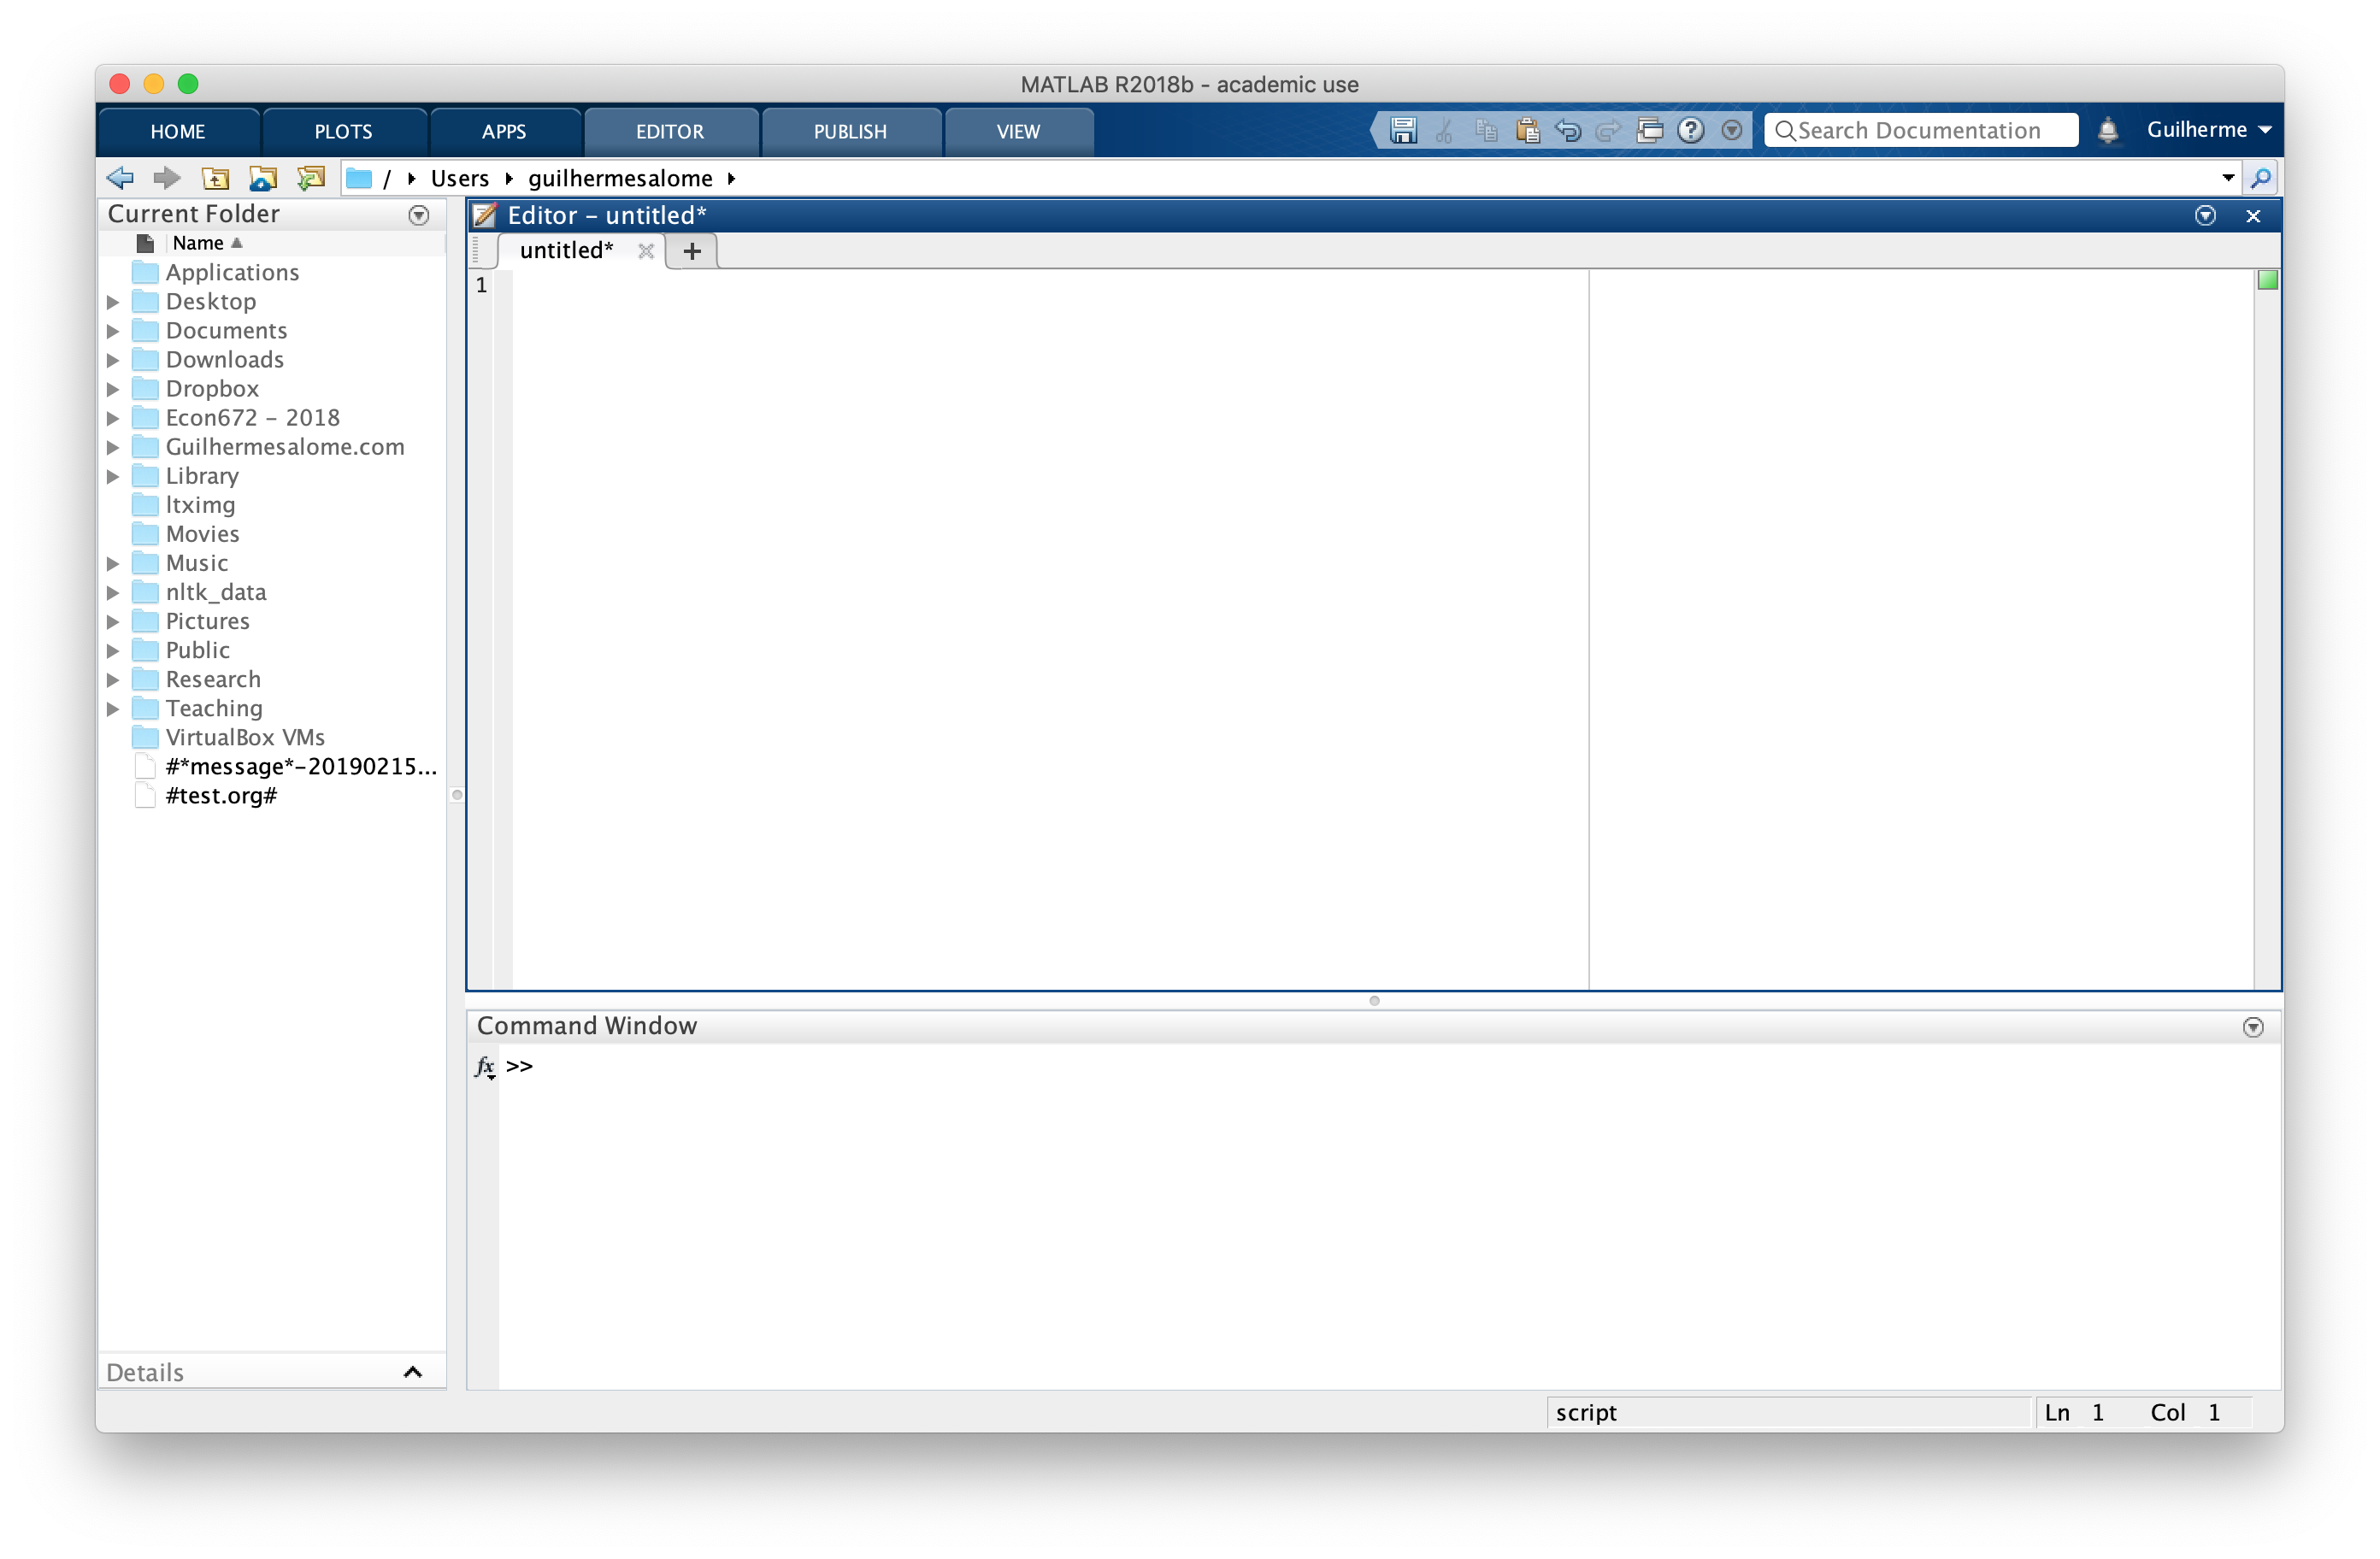
\includegraphics[width=.9\linewidth]{/Users/guilhermesalome/Teaching/Duke/Econ890 Matlab - 2019/supporting/matlab_ide_organized.png}
\caption{\label{fig:org8572d23}
A possible way to organize the windows in the IDE.}
\end{figure}

\section{Hello World!}
\label{sec:org185e86a}
We will now create a "hello world" program in Matlab.
Go on the \texttt{Editor} window and type the following:
\lstset{language=matlab,label= ,caption= ,captionpos=b,firstnumber=1,numbers=left,style=Matlab-editor}
\begin{lstlisting}
% helloworld.m
disp("Hello World!");
\end{lstlisting}
Save the file with a descriptive name, like \texttt{helloworld.m}.
Now, we would like to run our \texttt{helloworld.m} program.
There are two ways of doing so:
\begin{itemize}
\item Click on \texttt{Editor} and then on the green button \texttt{Run} (see Figure \ref{fig:org72d94dd});
\item Or, on the \texttt{Command Window} type the name of the file without the \texttt{.m} extension and hit enter.
\end{itemize}

\begin{figure}[!ht]
\centering
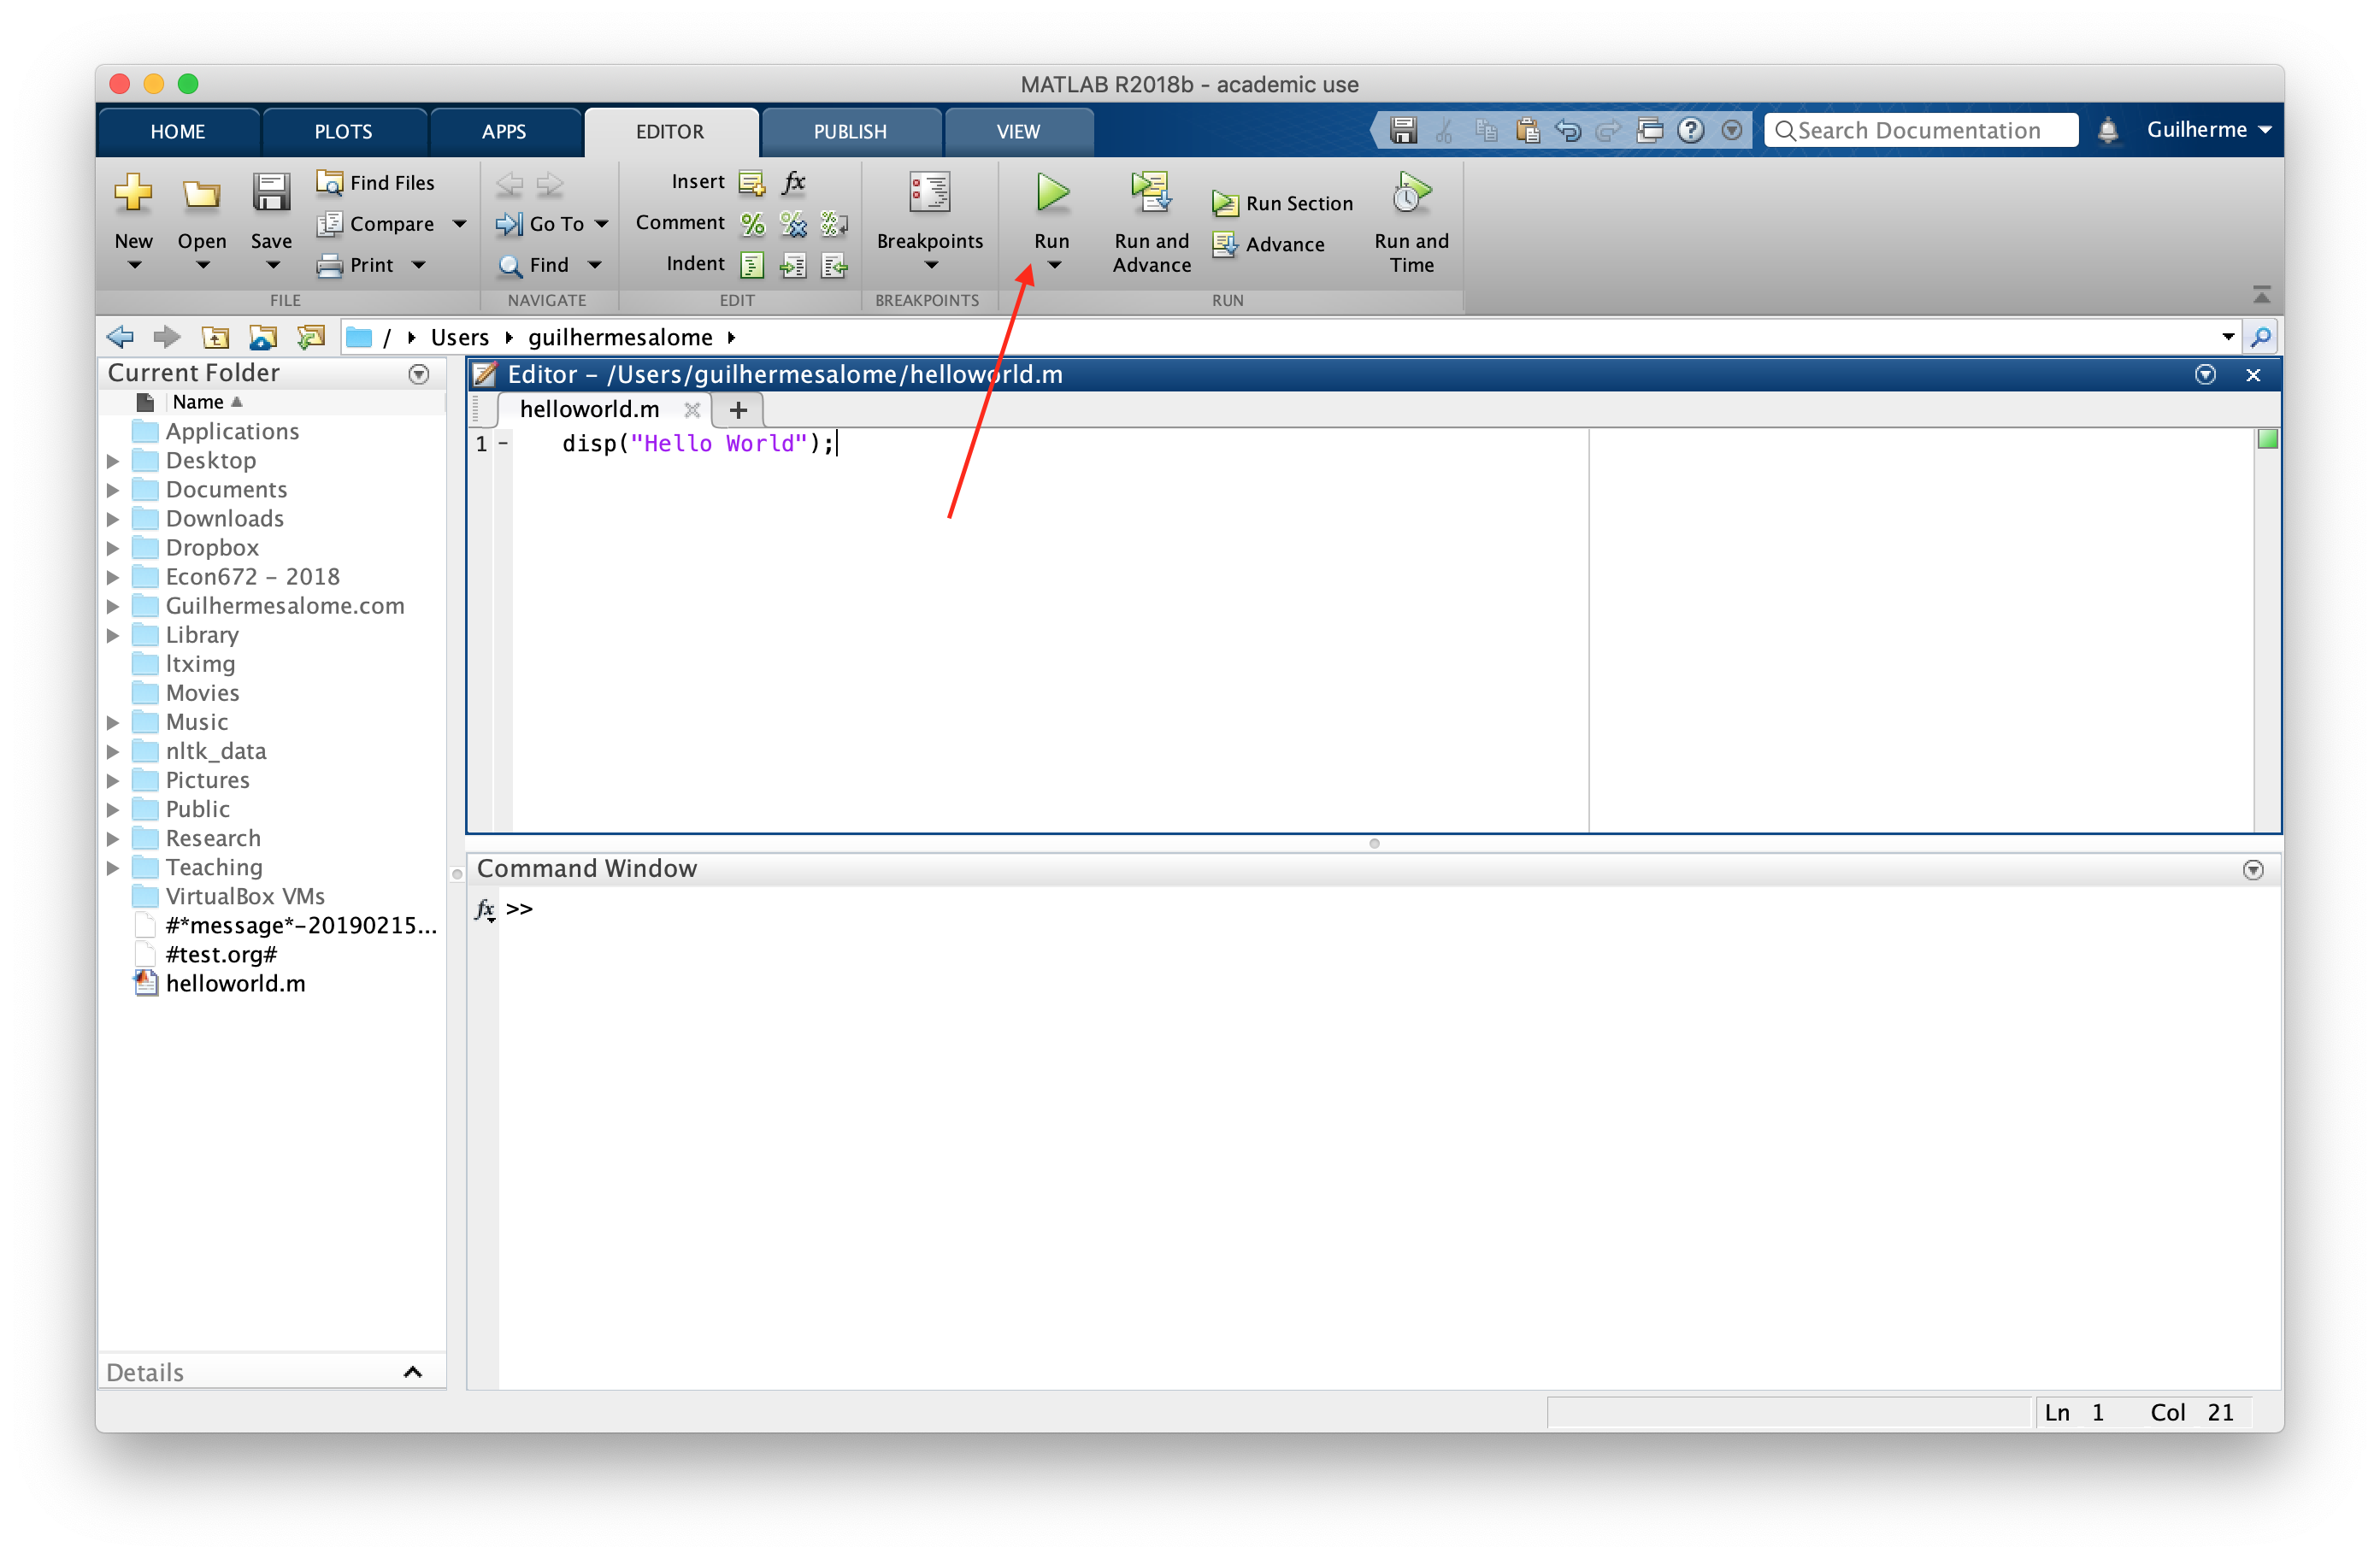
\includegraphics[width=.9\linewidth]{/Users/guilhermesalome/Teaching/Duke/Econ890 Matlab - 2019/supporting/matlab_helloworld_run.png}
\caption{\label{fig:org72d94dd}
Running a Matlab script.}
\end{figure}

When we run the file, Matlab displays the result in the \texttt{Command Window}.
The first line of the file starts with a percentage symbol, which indicates a comment line.
In the second line, the function \texttt{disp} is called.
This function takes a string as an argument and displays it on the screen.

\section{Linear Regression with Ordinary Least Squares}
\label{sec:org8e85dc9}
To learn the fundamentals of the Matlab programming language we will implement the ordinary least squares (OLS) estimator for the parameters of a linear regression under the classical assumptions.

Let's assume that the economic model of interest is given by:
\begin{align*}
\underbrace{y}_{n \times 1}=\underbrace{X}_{n\times K}\underbrace{\beta}_{K\times 1} + \underbrace{\varepsilon}_{n\times 1}
\end{align*}
where \(y\) is a \(n\times 1\) vector of observed dependent variables, \(X\) is an \(n \times K\) matrix of observed explanatory variables, \(\beta\) is a \(K\times 1\) vector of unknown parameters and \(\varepsilon\) is a \(n\times 1\) vector of unobserved explanatory variables.

We know that the OLS estimator of \(\beta\) (see Equation 1.2.5 in \citet{H2000}) is given by:
\begin{align*}
\hat{\beta}=(X'X)^{-1}X'y\numberthis\label{OLS_beta}
\end{align*}
Our first objective is to implement this estimator.

Using a bottom-up approach, we need to understand:
\begin{enumerate}
\item The data types for numbers in Matlab;
\item How to create vectors and matrices;
\item How to do matrix transposition, inversion and multiplication;
\item How to create a function that given \(X\) and \(y\) produces \(\hat{\beta}\);
\item How to generate data to test out our code.
\end{enumerate}

\subsection{Numeric Data Types for Numbers}
\label{sec:orga091203}
Numeric values are stored in the \href{https://en.wikipedia.org/wiki/Double-precision\_floating-point\_format}{double-precision floating point format}, by default.
The class name of this type of numeric value is \texttt{double}.
We can create doubles by simply assigning them to variables:
\lstset{language=matlab,label= ,caption= ,captionpos=b,firstnumber=1,numbers=left,style=Matlab-editor}
\begin{lstlisting}
x = 10;
y = 5
\end{lstlisting}
Whenever you see code in a box as above, you should run it yourself by typing the commands line by line, in the \texttt{Command Window}.

Notice that when the semicolon is omitted, Matlab displays the result of the assignment on the screen.
If you want to suppress this display you need the semicolon.
The use of semicolon is important when constructing scripts, so that the \texttt{Command Window} is not filled with information we do not need to see.
However, omitting the semicolon when typing in the \texttt{Command Window} is useful to see the result of operations.
\lstset{language=matlab,label= ,caption= ,captionpos=b,firstnumber=1,numbers=left,style=Matlab-editor}
\begin{lstlisting}
% The two lines below
y = 5;
disp(y);
% are equivalent to:
y = 5
\end{lstlisting}

The usual mathematical operations can be performed with numbers:
\lstset{language=matlab,label= ,caption= ,captionpos=b,firstnumber=1,numbers=left,style=Matlab-editor}
\begin{lstlisting}
x + y
x - y
% multiplication
x*y
% floating point division
y/x
x/y
% exponentiation
x^y
% remainder of integer division
mod(13, 5)
% integer division
floor(13/5)
% absolute value
abs(-1)
% maximum
max(x, y)
% minimum
min(x, y)
% exponential
exp(4)
% narutal logarithm
log(exp(1))
% square root
sqrt(4)
4^0.5
% factorial
factorial(x)
% pi
pi
sqrt(pi)
% trigonometry
sin(0)
cos(0)
tan(0)
\end{lstlisting}
The result of the operations above are still \texttt{double}.

You can verify the type and size in memory of a variable with the special\footnote{The function \texttt{whos} is being called with a special syntax called the \texttt{command syntax}. Usually, in a function call the parameters are passed inside parentheses, as in \texttt{mod(x, y)}. However, the \texttt{command syntax} allows us to pass parameters without using parentheses, as in \texttt{whos x y}. It is not often used, except with a few Matlab commands. More details about this \texttt{command syntax} are available at \href{https://www.mathworks.com/help/matlab/matlab\_prog/command-vs-function-syntax.html}{this page}.} function \texttt{whos}:
\lstset{language=matlab,label= ,caption= ,captionpos=b,firstnumber=1,numbers=left,style=Matlab-editor}
\begin{lstlisting}
whos x;
whos x y;
\end{lstlisting}

It is important to notice that the number displayed in the \texttt{Command Window} is a formatted version of the actual number stored in a variable.
For example, \(\pi\) is displayed as \(3.1416\).
By default, Matlab displays numbers using at most 5 digits, and it may use scientific notation for numbers that are too big or too small.
\lstset{language=matlab,label= ,caption= ,captionpos=b,firstnumber=1,numbers=left,style=Matlab-editor}
\begin{lstlisting}
pi
0.0000009809809
213124412123
\end{lstlisting}
We can change the \href{https://www.mathworks.com/help/matlab/matlab\_prog/display-format-for-numeric-values.html}{display format for numeric values} between 5 digits and 15 digits using the special command \texttt{format}:
\lstset{language=matlab,label= ,caption= ,captionpos=b,firstnumber=1,numbers=left,style=Matlab-editor}
\begin{lstlisting}
pi
% Use 15-digits to display numbers
format long;
pi
% Use 5-digits to display numbers
format short;
pi
% Force scientific notation with 5-digits
format short e;
pi
% Force scientific notation with 15-digits
format long e;
pi
\end{lstlisting}

Observe that, as with other implementations of \href{https://en.wikipedia.org/wiki/IEEE\_754}{floating-point arithmetic} (as in C or FORTRAN), Matlab is also subject to the usual rounding errors.
\lstset{language=matlab,label= ,caption= ,captionpos=b,firstnumber=1,numbers=left,style=Matlab-editor}
\begin{lstlisting}
3*(4/3 - 1) - 1
\end{lstlisting}
However, this is not a bug, but an issue resulting from not being possible to write \(\frac{4}{3}\) as a binary number using a finite number of bits.

There are other numeric types available, such as integers, complex numbers, infinity, not a number, among others.
It is worth mentioning that infinity and not a number can result from some arithmetic operations:
\lstset{language=matlab,label= ,caption= ,captionpos=b,firstnumber=1,numbers=left,style=Matlab-editor}
\begin{lstlisting}
% Finding infinity in Matlab
1/0
-1/0
% Not a number
1/0 - 1/0
\end{lstlisting}

Using \texttt{double} is sufficient for most applications, and for this reason we will skip the other numeric types.
However, applications that are memory bound or that require a lot of optimization may benefit from the other numeric types.
The official documentation on all numeric types is available on \href{https://www.mathworks.com/help/matlab/numeric-types.html}{this page}.
\subsection{Vectors and Matrices}
\label{sec:org5e54f2a}
Vectors and matrices are structured collections of numbers of type \texttt{double} (by default).
We can create vectors and matrices by:
\lstset{language=matlab,label= ,caption= ,captionpos=b,firstnumber=1,numbers=left,style=Matlab-editor}
\begin{lstlisting}
% A 5x1 vector
y = [10; -2; 3.4; exp(3); log(4.5)]
% A 5x3 matrix
X = [1, 2, 3;
     1,-3, 5;
     1, 4, 0;
     1, 0,-1;
     1, 4.5, 3.3]
\end{lstlisting}
Notice that commas separate columns and semicolons separate rows.
The use of commas to separate columns is optional.

We can very obtain the dimension of a vector with the function \texttt{length}, and the dimensions of a matrix with the function \texttt{size}:
\lstset{language=matlab,label= ,caption= ,captionpos=b,firstnumber=1,numbers=left,style=Matlab-editor}
\begin{lstlisting}
length(y)
size(X)
\end{lstlisting}
What would be the result of calling \texttt{length} on a matrix?
We can figure that out by reading the \texttt{help} documentation on the \texttt{length} function.
\lstset{language=matlab,label= ,caption= ,captionpos=b,firstnumber=1,numbers=left,style=Matlab-editor}
\begin{lstlisting}
help length
\end{lstlisting}
In the case of a matrix, it will return the value of the highest dimension.

Notice that the function \texttt{size} applied on a matrix returns two numbers.
We can access these two numbers separately by: saving them on two separate variables, or asking the function \texttt{size} to return only one of the numbers.
\lstset{language=matlab,label= ,caption= ,captionpos=b,firstnumber=1,numbers=left,style=Matlab-editor}
\begin{lstlisting}
A = ones(2, 3)
help size
% save the dimensions to two variables
[d1, d2] = size(A)
% ask size to return only the 1st dimension
d1 = size(A, 1)
% ask size to return only the 2nd dimension
d2 = size(A, 2)
\end{lstlisting}

To access the elements of vectors and matrices we use the following syntax:
\lstset{language=matlab,label= ,caption= ,captionpos=b,firstnumber=1,numbers=left,style=Matlab-editor}
\begin{lstlisting}
% The first element of a vector has the index 1
y(1)
% The second element of a vector has the index 2
y(2)
% And so on until the last element
y(5)
% For a matrix we need to define both dimensions
% The very first value at the first row and first column
X(1, 1)
% The value on the first row and second column
X(1, 2)
% The value on the last row and the last column
X(5, 3)
% There is a special syntax to get all rows of a column
X(:, 2) % all rows of 2nd column
X(:, 1) % all rows of 1st column
% The same notation applies to get all columns of a row
X(4, :) % all columns of the 4th row
X(1, :) % all columns of the 1st row
% We can use a similar notation to access slices of the matrix
X(2:4, 4) % rows 2 to 4 of the 4th column
X(3, 1:2) % columns 1 to 2 of the 3rd row
X(2:4, 1:2) % columns 1 to 2 of rows 2 to 4
\end{lstlisting}

The values stored in arrays (vectors, matrices and higher-dimensional matrices) can be modified in place:
\lstset{language=matlab,label= ,caption= ,captionpos=b,firstnumber=1,numbers=left,style=Matlab-editor}
\begin{lstlisting}
a = [0 1; 2 3]
a(2, 1) = 500
% multiple values can be updated at once
a(:, 1) = [30; 30] % modifying an entire column
a(2, :) = [20 20] % modifying an entire row
\end{lstlisting}

There are a few functions that assist in the creation of matrices:
\lstset{language=matlab,label= ,caption= ,captionpos=b,firstnumber=1,numbers=left,style=Matlab-editor}
\begin{lstlisting}
% Matrix full of zeros
help zeros
zeros(2)
zeros(4, 1)
% Matrix full of ones
ones(3)
ones(2, 3)
% Identity matrix
eye(5)
eye(2, 3)
% Sparse Identity Matrix
A = eye(1000)
B = speye(1000) % optimized
whos A B
% Diagonal matrix
diag([1 2 3 4 5])
\end{lstlisting}

We can also generate a vector by using a range of numbers:
\lstset{language=matlab,label= ,caption= ,captionpos=b,firstnumber=1,numbers=left,style=Matlab-editor}
\begin{lstlisting}
% start:stop
A = 1:4
% the values are incremented by 1 until the value is greater than
% the stop, which is 4
B = -5: 3.5
% we can change the increment using the syntax start:increment:stop
C = -5:0.5:3.5
\end{lstlisting}

We can combine other matrices to create new ones:
\lstset{language=matlab,label= ,caption= ,captionpos=b,firstnumber=1,numbers=left,style=Matlab-editor}
\begin{lstlisting}
A = [X(:, 1), X(:, 3)]
\end{lstlisting}
\subsection{Matrix Operations}
\label{sec:orgc264508}
We can now create matrices and modify them.
Now we will cover the \href{https://www.mathworks.com/help/matlab/math/basic-matrix-operations.html;jsessionid=e2359d161cc1539728b94fe2fea9}{basic matrix operations}.
Let's start with matrix and scalar operations:
\lstset{language=matlab,label= ,caption= ,captionpos=b,firstnumber=1,numbers=left,style=Matlab-editor}
\begin{lstlisting}
X = [1 2 3; 4 5 6]
% operations with a scalar are elementwise
X + 3
X - 2
% special notation for elementwise multiplication, division and exponentiation
X.*3
X./3
X.^3
% log, exp and sqrt apply elementwise
log(X)
exp(X)
sqrt(X)
\end{lstlisting}

Matrix and matrix operations:
\lstset{language=matlab,label= ,caption= ,captionpos=b,firstnumber=1,numbers=left,style=Matlab-editor}
\begin{lstlisting}
A = [10 20 30; 0 -5 -10];
B = [2 2 2; 5 10 20];
% elementwise operations (matrices have the same dimensions)
A + B
A - B
A./B
A.*B
% concatenation
% concatenate rows (vertical concatenation)
C = vertcat(A, B)
C = [A; B]
% concatenate columns (horizontal concatenation)
D = horzcat(A, B)
D = [A B]
% repetition
repmat(A, 2, 3) % repeats matrix A: 2 times in row, 3 times in column
\end{lstlisting}

Now, for linear algebra:
\lstset{language=matlab,label= ,caption= ,captionpos=b,firstnumber=1,numbers=left,style=Matlab-editor}
\begin{lstlisting}
A = [10 2 30;
     0 -5 -10]
B = ones(size(A, 2), 1)
% Matrix multiplication
C = A*B
% Matrix tranposition
transpose(A)
A'
% Matrix inversion
C = [A; B']
C^(-1)
inv(C)
% Solving linear system Cx=B
solution = C\B
% Eigenvalues and eigenvectors
eigenvalues = eig(C)
[eigenvectors, eigenvalues] = eig(C)
% Singular value decomposition
[U, S, V] = svd(C)
% Kronecker Product
kron(A, B)
\end{lstlisting}
There are many other useful linear algebra functions.
The full documentation is available on \href{https://www.mathworks.com/help/matlab/linear-algebra.html?s\_tid=CRUX\_lftnav}{the linear algebra reference page}.
\subsection{Functions (and Conditionals)}
\label{sec:orgbd4f478}
We now have the main ingredients to implement the OLS estimator from Equation \ref{OLS_beta}:
\lstset{language=matlab,label= ,caption= ,captionpos=b,firstnumber=1,numbers=left,style=Matlab-editor}
\begin{lstlisting}
y = [10; -2; 3.4; exp(3); log(4.5)]
X = [1, 2, 3;
     1,-3, 5;
     1, 4, 0;
     1, 0,-1;
     1, 4.5, 3.3]
% The OLS estimator for the regression y = X*beta + epsilon
beta_hat = inv(X'*X)*X'*y
\end{lstlisting}
Now that we have the estimator, we want to be able to use it for whatever matrices \(X\) and \(y\) we have.
To do that, we create a function.

\href{https://www.mathworks.com/help/matlab/ref/function.html}{Functions} in Matlab are created in separate files ending in \texttt{.m}.
Each function has its own \texttt{.m} file\footnote{Strictly speaking there can be more than one function in a single \texttt{.m} file, but there must be one function with the same name as the file name, and the other functions in the file are known as local functions. These local functions are not available outside of the \texttt{.m} file, and their use is to break down the code in smaller pieces.}.
The syntax for a function is \texttt{function [output1, ..., outputN] = foo(input1, ..., inputM)}, then the actual function code, and last we finish with the keyword \texttt{end}.
Let's create a simple function for the OLS estimator:
\lstset{language=matlab,label= ,caption= ,captionpos=b,firstnumber=1,numbers=left,style=Matlab-editor}
\begin{lstlisting}
% linreg_ols.m
function [beta] = linreg_ols(y, X)
beta = inv(X'*X)*X'*y;
end
\end{lstlisting}
Whenever you see a box as above where the first line starts with a comment of the type \texttt{\% somename.m}, it means that you should type the code in a new file and save it with the name given in the comment.
Save the file on the current folder Matlab is using.

Notice that the name of the function \uline{must} be the same name of the file.
After saving the file, we can use the function by just calling its name:
\lstset{language=matlab,label= ,caption= ,captionpos=b,firstnumber=1,numbers=left,style=Matlab-editor}
\begin{lstlisting}
beta = linreg_ols(y, X)
\end{lstlisting}
Matlab can access all \texttt{.m} files in the current folder and on sub-folders within it.\footnote{It is possible to use functions and other files in folders outside the current folder. To do so, you need to add the path to that specific folder to the search path Matlab uses. This can be done with the function \texttt{addpath}. See the \href{https://www.mathworks.com/help/matlab/ref/addpath.html}{\texttt{addpath} reference} for details.}

There are a couple of modifications we need to do to the \texttt{linreg\_ols} function.
First, we need to add documentation about it, so that our future selves know what it actually does.
We do so by adding comments to the function right after the line where the function is declared.
These comments should accomplish the following:
\begin{itemize}
\item A description of the function does in one line (or very few lines);
\item A description of the function inputs;
\item A description of the function outputs;
\item Examples of usage.
\end{itemize}
After finishing core functions it is absolutely necessary to add documentation.
If you stop using your code, even for a few days, it is very easy to forget what you did and what different functions do.
Having the documentation is fundamental to quickly remember how to operate your code.
We can add comments in Matlab with a percentage symbol.
Let's add comments so that the usage of the function is clear:
\lstset{language=matlab,label= ,caption= ,captionpos=b,firstnumber=1,numbers=left,style=Matlab-editor}
\begin{lstlisting}
% linreg_ols.m
function [beta] = linreg_ols(y, X)
% LINREG_OLS estimates beta in the linear regression y = X*beta + epsilon
% via ordinary least squares
%
% Args:
%     y: A nx1 vector of dependent variables
%     X: A nxK matrix of independent variables
%
% Returns:
%     beta: A Kx1 vector of the estimated beta coefficients
%
% Examples:
%     y = [1;2;3];
%     X = rand(3);
%     beta = linreg_ols(y, X)
%
% Reference:
% Equation 1.2.5 in Hayashi, F. (2010).
% Econometrics. Princeton University Press. isbn: 9780691010182.

beta = inv(X'*X)*X'*y;

end
\end{lstlisting}
You can see the documentation of the function with the special command \texttt{help}.
\lstset{language=matlab,label= ,caption= ,captionpos=b,firstnumber=1,numbers=left,style=Matlab-editor}
\begin{lstlisting}
help linreg_ols
\end{lstlisting}

Often we want to add an intercept to the linear regression.
Let's extend our \texttt{linreg\_ols} function to automatically add an intercept.
To conserve space in the lecture notes, I will remove the documentation for our function, but you should not.
\lstset{language=matlab,label= ,caption= ,captionpos=b,firstnumber=1,numbers=left,style=Matlab-editor}
\begin{lstlisting}
% linreg_ols.m
function [beta] = linreg_ols(y, X)
% add intercept to X
X = horzcat(ones(size(X, 1), 1), X); % X is a local variable to this function
beta = inv(X'*X)*X'*y;
end
\end{lstlisting}

If we want the intercept to be optional, then we need to add a new input to the function that will represent whether or not we want the intercept to be added to \(X\).
We can do so by using the conditional statement \texttt{if}.
\subsubsection{Conditionals}
\label{sec:org98d0d16}
The syntax for conditional statements is:
\lstset{language=matlab,label= ,caption= ,captionpos=b,firstnumber=1,numbers=left,style=Matlab-editor}
\begin{lstlisting}
if condition
    % code to run if condition is true
elseif another_condition
    % code to run if condition is false and
    % another_condition is true
else
    % code to run if condition and another_condition are false
end
\end{lstlisting}

In this case the \texttt{condition} is pretty simple, we can add an input with the name \texttt{add\_intercept} and if its value is \texttt{true} we add the intercept, otherwise we do not.
In Matlab, the possible logical (boolean) values are \texttt{true} and \texttt{false}, but the numbers \texttt{1} and \texttt{0} can also be used to the same extent.
The basic relational operators are:
\lstset{language=matlab,label= ,caption= ,captionpos=b,firstnumber=1,numbers=left,style=Matlab-editor}
\begin{lstlisting}
% equal to
true == 1
% not equal to
true ~= false
% greater than
3 > 2
% greater or equal than
2 >= 2
% less than
3 < 2
% less or equal than
-1 <= 0
\end{lstlisting}

It is also possible to combine different conditions with these logical operators:
\lstset{language=matlab,label= ,caption= ,captionpos=b,firstnumber=1,numbers=left,style=Matlab-editor}
\begin{lstlisting}
% and
(1 > 0) && (2 > 1)
% or
(1 < 0) || (2 < 1)
% not
~(1 > 0)
\end{lstlisting}
\subsubsection{Optional Intercept}
\label{sec:orgfc351d1}
Let's modify \texttt{linreg\_ols} to make the intercept optional:
\lstset{language=matlab,label= ,caption= ,captionpos=b,firstnumber=1,numbers=left,style=Matlab-editor}
\begin{lstlisting}
% linreg_ols.m
function [beta] = linreg_ols(y, X, add_intercept)
if add_intercept:
    X = horzcat(ones(size(X, 1), 1), X);
end
beta = inv(X'*X)*X'*y;
end
\end{lstlisting}

Finally, we update the documentation:
\lstset{language=matlab,label= ,caption= ,captionpos=b,firstnumber=1,numbers=left,style=Matlab-editor}
\begin{lstlisting}
% linreg_ols.m
function [beta] = linreg_ols(y, X, add_intercept)
% LINREG_OLS estimates beta in the linear regression y = X*beta + epsilon
% via ordinary least squares
%
% Args:
%     y: A nx1 vector of dependent variables
%     X: A nxK matrix of independent variables
%     add_intercept: A boolean variable. If true, then a column of
%        ones is added to X, so that an intercept for the linear
%        regression is estimated.
%
% Returns:
%     beta: A Kx1 vector of the estimated beta coefficients
%
% Examples:
%     y = [1;2;3];
%     X = rand(3);
%     beta = linreg_ols(y, X)
%
% Reference:
% Equation 1.2.5 in Hayashi, F. (2010).
% Econometrics. Princeton University Press. isbn: 9780691010182.
if add_intercept:
    X = horzcat(ones(size(X, 1), 1), X);
end
beta = inv(X'*X)*X'*y;
end
\end{lstlisting}
\subsection{Generating Data (and Loops and Text)}
\label{sec:org2098963}
To test if our function is actually doing what we think it is doing, we need to test it.
Testing is imperative when programming, since generating code that is 100$\backslash$% correct the first time is quite hard.

In this case, we are going to simulate data for \(X\), \(\varepsilon\) and \(y\), while fixing true values for the parameters \(\beta\).
First, to simulate the data we will assume that
In Matlab, the \href{https://www.mathworks.com/help/matlab/random-number-generation.html}{basic random number generation} functions can generate values from the uniform and normal distributions.
However, in the "Statistics and Machine Learning Toolbox" there are \href{https://www.mathworks.com/help/stats/random-number-generation.html}{random number generators for many other distributions}.
Let's assume \(X\) comes from the uniform distribution on the interval \((0, 1)\), while \(\varepsilon\) comes from the standard normal distribution.
We will generate these values in a loop.

\subsubsection{Loops}
\label{sec:org2d3b01d}
In Matlab, we can create \texttt{for} loops and \texttt{while} loops.
The syntax for \texttt{for} loops is:
\lstset{language=matlab,label= ,caption= ,captionpos=b,firstnumber=1,numbers=left,style=Matlab-editor}
\begin{lstlisting}
% syntax for for loops
for variable = range
    % variable takes the value in the range
    % run some code
end
% example
for i = 1:10
    disp(i)
end
% example with nested loops
X = zeros(3)
for i = 1:size(X, 1)
    for j = 1:size(X, 2)
        X(i, j) = i + j;
    end
end
\end{lstlisting}
For loops will terminate when all values in the range are exhausted.

The syntax for \texttt{while} loops is similar:
\lstset{language=matlab,label= ,caption= ,captionpos=b,firstnumber=1,numbers=left,style=Matlab-editor}
\begin{lstlisting}
% syntax for while loops
while condition
    % if condition is true
    % run some code
end
% the condition must be a boolean value

% example
i = 0
while i < 10
    disp(i)
    i = i + 1 % no i++ or += on Matlab
end
\end{lstlisting}
While loops will terminate when the condition is no longer true.

If you write an infinite loop, you can break out of it with \texttt{Ctrl + C}.
In addition, if you need a loop to terminate earlier you can use the keyword \texttt{break}.
For example:
\lstset{language=matlab,label= ,caption= ,captionpos=b,firstnumber=1,numbers=left,style=Matlab-editor}
\begin{lstlisting}
numb_iter = 0
max_iter = 10
distance = 1000
while distance > 0.01
    distance = distance/2
    if numb_iter >= max_iter
        disp("I will break now")
        break
    else
        numb_iter = numb_iter + 1
    end
end
\end{lstlisting}
\subsubsection{Generating Data in a Loop}
\label{sec:orgc3bc6fb}
Let's now create our test data.
We will generate a matrix \(X\) with 100 rows and 5 columns, and \(\varepsilon\) will be a vector with 100 rows.
We will create this data in a script, so that we can run it multiple times with different number of rows and columns.
\lstset{language=matlab,label= ,caption= ,captionpos=b,firstnumber=1,numbers=left,style=Matlab-editor}
\begin{lstlisting}
% script: test_linreg_ols.m
% Generates data from the linear model y = X*beta + epsilon,
% given the true beta values. Estimates beta using the function
% linreg_ols and displays a table comparing true values to
% parameters.

% number of rows and columns
nrows = 100;
ncols = 5;
% true betas
beta = [-1; 2; 0.5; 3; 0.1];
% generate data for X, epsilon and y
X = zeros(nrows, ncols);
epsilon = zeros(nrows, 1);
y = zeros(nrows, 1);
for i = 1:nrows
    X(i, :) = rand(1, 5);
    epsilon(i) = randn();
    y(i) = X(i,:)*beta + epsilon(i);
end
% estimate the betas from X and y
beta_hat = linreg_ols(y, X, true);
\end{lstlisting}
Whenever we run the script above, we will generate data and estimate the values of \(\beta\).
Notice that we added an intercept in the estimation, even though the true model does not have an intercept.
To make the comparison between true parameters values and their estimates, we would like to display the values side by side, with some text indicating what are the true parameters and what are the estimates.
\subsubsection{Characters and Strings}
\label{sec:org5685062}
In Matlab, there are \href{https://www.mathworks.com/help/matlab/characters-and-strings.html}{two data types for text}: \texttt{char} and \texttt{string}.
A \texttt{char} holds a sequence of characters.
It works like a vector of numbers, but holds characters instead.
To create a \texttt{char} we use single quotes \texttt{'}:
\lstset{language=matlab,label= ,caption= ,captionpos=b,firstnumber=1,numbers=left,style=Matlab-editor}
\begin{lstlisting}
name = 'Guilherme'
% name is an array of characters, the individual letters of my name
length(name)
name(1)
name(length(name))
% we can also concatenate character arrays
disp(['My name is ' name '!'])
\end{lstlisting}
Characters are meant to store short pieces of text, and are used to specify file names, labels and titles for plots, and inputs for functions.

A \texttt{string} array is meant to hold and manipulate larger pieces of text.
Matlab provides various functions for manipulating text stored in \texttt{string} arrays.
String arrays are created in a fashion similar to matrices, but with brackets and text in double quotes \texttt{"}:
\lstset{language=matlab,label= ,caption= ,captionpos=b,firstnumber=1,numbers=left,style=Matlab-editor}
\begin{lstlisting}
% creating a simple string array
full_name = ["Guilherme", "Salome"];
% full_name is a string array
size(full_name)
full_name(1, 1)
full_name(1, 2)
% a string array with many rows and columns
students_names = ["First Name", "Last Name";
                  "A", "B";
                  "C", "D"];
size(students_names)
students_names(2, 2)
% a string array can also contain a single element
% in this case, we do not need the brackets
my_name = "Guilherme Salome"
size(my_name) % it is still an array
% we can find the length of a string with the strlength function
strlength(my_name)
% creating a string array that also has numbers will
% implicitely convert numbers to strings
data = ["Parameters", 1, 2, 3];
\end{lstlisting}

Let's explore some of the common operations we might perform with strings.
A full list of functions that operate on strings are available on the \href{https://www.mathworks.com/help/matlab/characters-and-strings.html}{reference page for characters and strings}.
\lstset{language=matlab,label= ,caption= ,captionpos=b,firstnumber=1,numbers=left,style=Matlab-editor}
\begin{lstlisting}
% we can append a string to string arrays
first_names = ["Mary", "John", "Paul"]
full_names = first_names + " Smith"
% split strings
split_sentence = split("This is a sentence about to be split")
% split can be used to clean csv data
csv_data = "1.2, 3.2, -0.5, 5.3"
split_data = split(csv_data, ',')
% join strings
a_burguer = join(["Bread", "Tomato", "Lettuce", "Burguer", "Cheese", ...
                  "Bread"])
% if a command is too big for a single line, we can use
% the ... notation to continue it in the next line

% joining strings can be useful to store data in the csv file
data = [1.2; 3.2; -0.5; 5.3];
% the text manipulation functions apply to string arrays
% so we need to convert the numbers to a string array
data_string = string(data)
csv_data = join(data_string, ',')
% sorting strings
sort(full_names)
\end{lstlisting}

We can now display our parameter estimates using string arrays:
\lstset{language=matlab,label= ,caption= ,captionpos=b,firstnumber=1,numbers=left,style=Matlab-editor}
\begin{lstlisting}
% compare the true betas to the estimates
disp(horzcat(["True Values"; 0; beta], ["Estimates"; beta_hat]))
\end{lstlisting}
\subsubsection{Table}
\label{sec:orgfdb5cb0}
We can create a better display by using a \href{https://www.mathworks.com/help/matlab/ref/table.html\#d117e1339894}{\texttt{table}}.
A \texttt{table} contains rectangular data that is column-oriented.
We can create a table to display the true parameter values and their estimates.
We create a table by passing it vectors with the values, each vector will be a column in the table.
Additionally, we can pass a string array containing the column names.
\lstset{language=matlab,label= ,caption= ,captionpos=b,firstnumber=1,numbers=left,style=Matlab-editor}
\begin{lstlisting}
% script: test_linreg_ols.m
% Generates data from the linear model y = X*beta + epsilon,
% given the true beta values. Estimates beta using the function
% linreg_ols and displays a table comparing true values to
% parameters.

% number of rows and columns
nrows = 100;
ncols = 5;
% true betas
beta = [-1; 2; 0.5; 3; 0.1];
% generate data for X, epsilon and y
X = zeros(nrows, ncols);
epsilon = zeros(nrows, 1);
y = zeros(nrows, 1);
for i = 1:nrows
    X(i, :) = rand(1, 5);
    epsilon(i) = randn();
    y(i) = X(i,:)*beta + epsilon(i);
end
% estimate the betas from X and y
beta_hat = linreg_ols(y, X, true);
% display a table with the true parameters and estimates
estimates = table([0; beta], beta_hat, 'VariableNames', ["Parameters", ...
                    "Estimates"]);
disp(estimates)
\end{lstlisting}

We can now modify this script to see what happens to the estimates when the number of data points increases, or when the number of parameters increases and so on.
We have covered most of the basics of Matlab by coding the \texttt{linreg\_ols} function and the \texttt{test\_linreg\_ols.m} script.
\section{Standard Errors for OLS Estimates}
\label{sec:orgf65fa21}
We will now extended the \texttt{linreg\_ols} function to compute standard errors for the parameter estimates and the t-statistics.

Under the classical assumptions, the standard error of the OLS estimates (Equation 1.4.4 in \citet{H2000}) is given by:
\begin{align*}
SE(\hat{\beta}_i) = \sqrt{s^2\cdot[(X'X)^{-1}]_{[i, i]}}
\end{align*}
where \(s^2\) (Equation 1.2.13 in \citet{H2000}) is computed from the residuals of the estimation:
\begin{align*}
e&\equiv y-X\hat{\beta}\\
s^2&\equiv\frac{e'e}{n-K}
\end{align*}
Let's implement this estimator in the \texttt{linreg\_ols} function:
\lstset{language=matlab,label= ,caption= ,captionpos=b,firstnumber=1,numbers=left,style=Matlab-editor}
\begin{lstlisting}
% linreg_ols.m
function [beta, s2, stderr] = linreg_ols(y, X, add_intercept)
% Returns:
%     beta: A Kx1 vector of the estimated beta coefficients
%     s2: Estimate of the residual variance
%     stderr: A Kx1 vector of the estimators of the standard errors
%        of the beta estimates
if add_intercept
    X = horzcat(ones(size(X, 1), 1), X);
end
% compute inv(X'X) just once (used multiple times)
XX = X'*X;
% equivalent to inv(X'X) but faster and more numerically stable
XXinverse = XX\eye(length(XX));
beta = XXinverse*X'*y;
% estimate Var(beta_hat|X)
e = y - X*beta;
s2 = (e'*e)/(size(X, 1) - size(X, 2));
stderr = diag((s2*XXinverse)^0.5);
end
\end{lstlisting}
Now, the t-statistic for the null-hypothesis of insignificant coefficients is:
\begin{align*}
t_i\equiv\frac{\hat{\beta}_i}{SE(\hat{\beta}_i)}\sim t_{n-K}
\end{align*}
To compute the p-value for the test (see Pages 38 and 39 of \citet{H2000}) we need the cumulative density function (cdf) of the student's T distribution, which is available in the function \texttt{tcdf}.
\lstset{language=matlab,label= ,caption= ,captionpos=b,firstnumber=1,numbers=left,style=Matlab-editor}
\begin{lstlisting}
% linreg_ols.m
function [beta, s2, stderr, t_stat, p_value] = linreg_ols(y, X, add_intercept)
% LINREG_OLS estimates beta in the linear regression y = X*beta + epsilon
% via ordinary least squares
%
% Args:
%     y: A nx1 vector of dependent variables
%     X: A nxK matrix of independent variables
%     add_intercept: A boolean variable. If true, then a column of
%        ones is added to X, so that an intercept for the linear
%        regression is estimated.
%
% Returns:
%     beta: A Kx1 vector of the estimated beta coefficients
%     s2: Estimate of the residual variance
%     stderr: A Kx1 vector of the estimators of the standard errors
%        of the beta estimates
%     t_stat: A Kx1 vector with the t-statistics for the null
%        hypothesis that each beta is zero (separately)
%     p_value: A Kx1 vector with the p-values for the t-test
%
% Examples:
%     y = [1;2;3];
%     X = rand(3);
%     beta = linreg_ols(y, X, true)
%
% Reference:
% Equation 1.2.5 in Hayashi, F. (2010).
% Econometrics. Princeton University Press. isbn: 9780691010182.
if add_intercept
    X = horzcat(ones(size(X, 1), 1), X);
end
% compute inv(X'X) just once (used multiple times)
XX = X'*X;
% equivalent to inv(X'X) but faster and more numerically stable
XXinverse = XX\eye(length(XX));
% number of observations and explanatory variables
n = size(X, 1);
K = size(X, 2);
beta = XXinverse*X'*y;
% estimate Var(beta_hat|X)
e = y - X*beta;
s2 = (e'*e)/(n - K);
stderr = diag((s2*XXinverse)^0.5);
% t-statistics
t_stat = beta./stderr;
p_value = (1 - tcdf(abs(t_stat), n - K))*2;
end
\end{lstlisting}
\section{Organizing the Regression Results in an Object}
\label{sec:orgd585d39}
We could further extend the \texttt{linreg\_ols} function to compute all the other statistics commonly found in other specialized statistics software.
Every time we add a new computation to the function, we would have to extend the number of outputs.
When there are too many outputs in a function, we need a better way to organize them.
To organize multiple outputs of a function we can use a \href{https://www.mathworks.com/help/matlab/ref/struct.html}{\texttt{struct}}.

A \texttt{struct} (structure array) is a data type that groups other data by fields.
Each field has a name and can contain any type of data.
We access fields in a structure array with the \texttt{.} notation.
Let's create a simple \texttt{struct}:
\lstset{language=matlab,label= ,caption= ,captionpos=b,firstnumber=1,numbers=left,style=Matlab-editor}
\begin{lstlisting}
% data to store
beta_hat = [1;2;3];
stderr = [0.5, 0.3, 0.43];
% create a structure named results
results.b = beta_hat;
results.se = stderr;
% access the values in the struct
results.b
results.se
% creating a struct using the struct keyword
results = struct('b', beta_hat, 'se', stderr);
results.b
results.se
% creating a struct with empty fields (possibly to be filled later)
results = struct('b', [], 'se', []);
results.b
results.b = beta_hat;
results.b
\end{lstlisting}

We can use a \texttt{struct} to easily organize the output of \texttt{linreg\_ols}:
\lstset{language=matlab,label= ,caption= ,captionpos=b,firstnumber=1,numbers=left,style=Matlab-editor}
\begin{lstlisting}
% linreg_ols.m
function results = linreg_ols(y, X, add_intercept)
% LINREG_OLS estimates beta in the linear regression y = X*beta + epsilon
% via ordinary least squares
%
% Args:
%     y: A nx1 vector of dependent variables
%     X: A nxK matrix of independent variables
%     add_intercept: A boolean variable. If true, then a column of
%        ones is added to X, so that an intercept for the linear
%        regression is estimated.
%
% Returns:
%     results: A struct with the following fields:
%       beta: A Kx1 vector of the estimated beta coefficients
%       s2: Estimate of the residual variance
%       stderr: A Kx1 vector of the estimators of the standard
%       errors of the beta estimates
%       t_stat: A Kx1 vector with the t-statistics for the null
%          hypothesis that each beta is zero (separately)
%       p_value: A Kx1 vector with the p-values for the t-test
%
% Examples:
%     y = [1;2;3];
%     X = rand(3);
%     beta = linreg_ols(y, X, true)
%
% Reference:
% Equation 1.2.5 in Hayashi, F. (2010).
% Econometrics. Princeton University Press. isbn: 9780691010182.
if add_intercept
    X = horzcat(ones(size(X, 1), 1), X);
end
% compute inv(X'X) just once (used multiple times)
XX = X'*X;
% equivalent to inv(X'X) but faster and more numerically stable
XXinverse = XX\eye(length(XX));
% number of observations and explanatory variables
n = size(X, 1);
K = size(X, 2);
beta = XXinverse*X'*y;
% estimate Var(beta_hat|X)
e = y - X*beta;
s2 = (e'*e)/(n - K);
stderr = diag((s2*XXinverse)^0.5);
% t-statistics
t_stat = beta./stderr;
p_value = (1 - tcdf(abs(t_stat), n - K))*2;
% create results struct
results = struct('b', beta, 's2', s2, 'stderr', stderr, ...
                 't_stat', t_stat, 'p_value', p_value);
end
\end{lstlisting}
While a \texttt{struct} can be very useful to organize data, it is not the fastest data type available in Matlab and should not be overused.
\section{Validating Input and Debugging}
\label{sec:orgf32519d}
The \texttt{linreg\_ols} function is well documented and provides the bare bones for linear regressions.
However, it is missing input validation.
What should \texttt{linreg\_ols} return if the matrix \(X\) has more columns than lines?
Or if \(y\) and \(X\) do not have the same number of rows?
\subsection{Validating Input}
\label{sec:org535d91b}
We can validate data with conditionals, and if something fails the validation, we throw an error.
In Matlab, we can throw an error with the function \href{https://www.mathworks.com/help/matlab/ref/error.html}{\texttt{error}}, which takes a string as input and displays it to the user while interrupting the execution of the code.
We can add the following lines to the beginning of the \texttt{linreg\_ols} function:
\lstset{language=matlab,label= ,caption= ,captionpos=b,firstnumber=1,numbers=left,style=Matlab-editor}
\begin{lstlisting}
% linreg_ols.m
function results = linreg_ols(y, X, add_intercept)
%% Input validation
if size(y, 1) ~= size(X, 1)
    error("y and X have a different number of rows")
end
if size(X, 1) < size(X, 2)
    error("X has less rows than columns")
end
%% Code to run after inputs are validated ...
end
\end{lstlisting}
If the inputs fail the validation, the code is interrupted and a message is displayed in red so that the user can take action to fix the issues.
It is important that the message is clear and identifies the issue as directly as possible.

Observe the use of two percentage symbols instead of one.
Lines that start with \texttt{\%\%} are also comments, but Matlab consider these lines as the start of a section.
A section is just a tool to organize code in \texttt{.m} files and has no effect on the code.

Now, what happens if we forget to specify whether we want an intercept?
That is, we execute \texttt{linreg\_ols(y, X)}.
In this case, \texttt{add\_intercept} is a required input, so Matlab will warn you that there are not enough input arguments.
We can see what happens in detail by using the \texttt{debugging} features Matlab provides.
\subsection{Debugging}
\label{sec:org7d74e88}
\href{https://www.mathworks.com/help/matlab/matlab\_prog/debugging-process-and-features.html}{Debugging} in the Matlab IDE is done by setting breakpoints, and then executing your code normally.
When the code reaches a breakpoint, the execution is paused and you have access to the variables available at that point in your code.
You can then choose to continue executing the code in different ways.
You can continue the execution line by line, continue until where the cursor is at, or continue until the code finishes or finds another breakpoint.

You can add a breakpoint by clicking right next to the number line in the code editor.
See Figure \ref{fig:org71a5a7e} on how to add a breakpoint.
When you click a red circle will show up indicating that a breakpoint was added.
You can remove breakpoints by clicking on the red circles.

\begin{figure}[!ht]
\centering
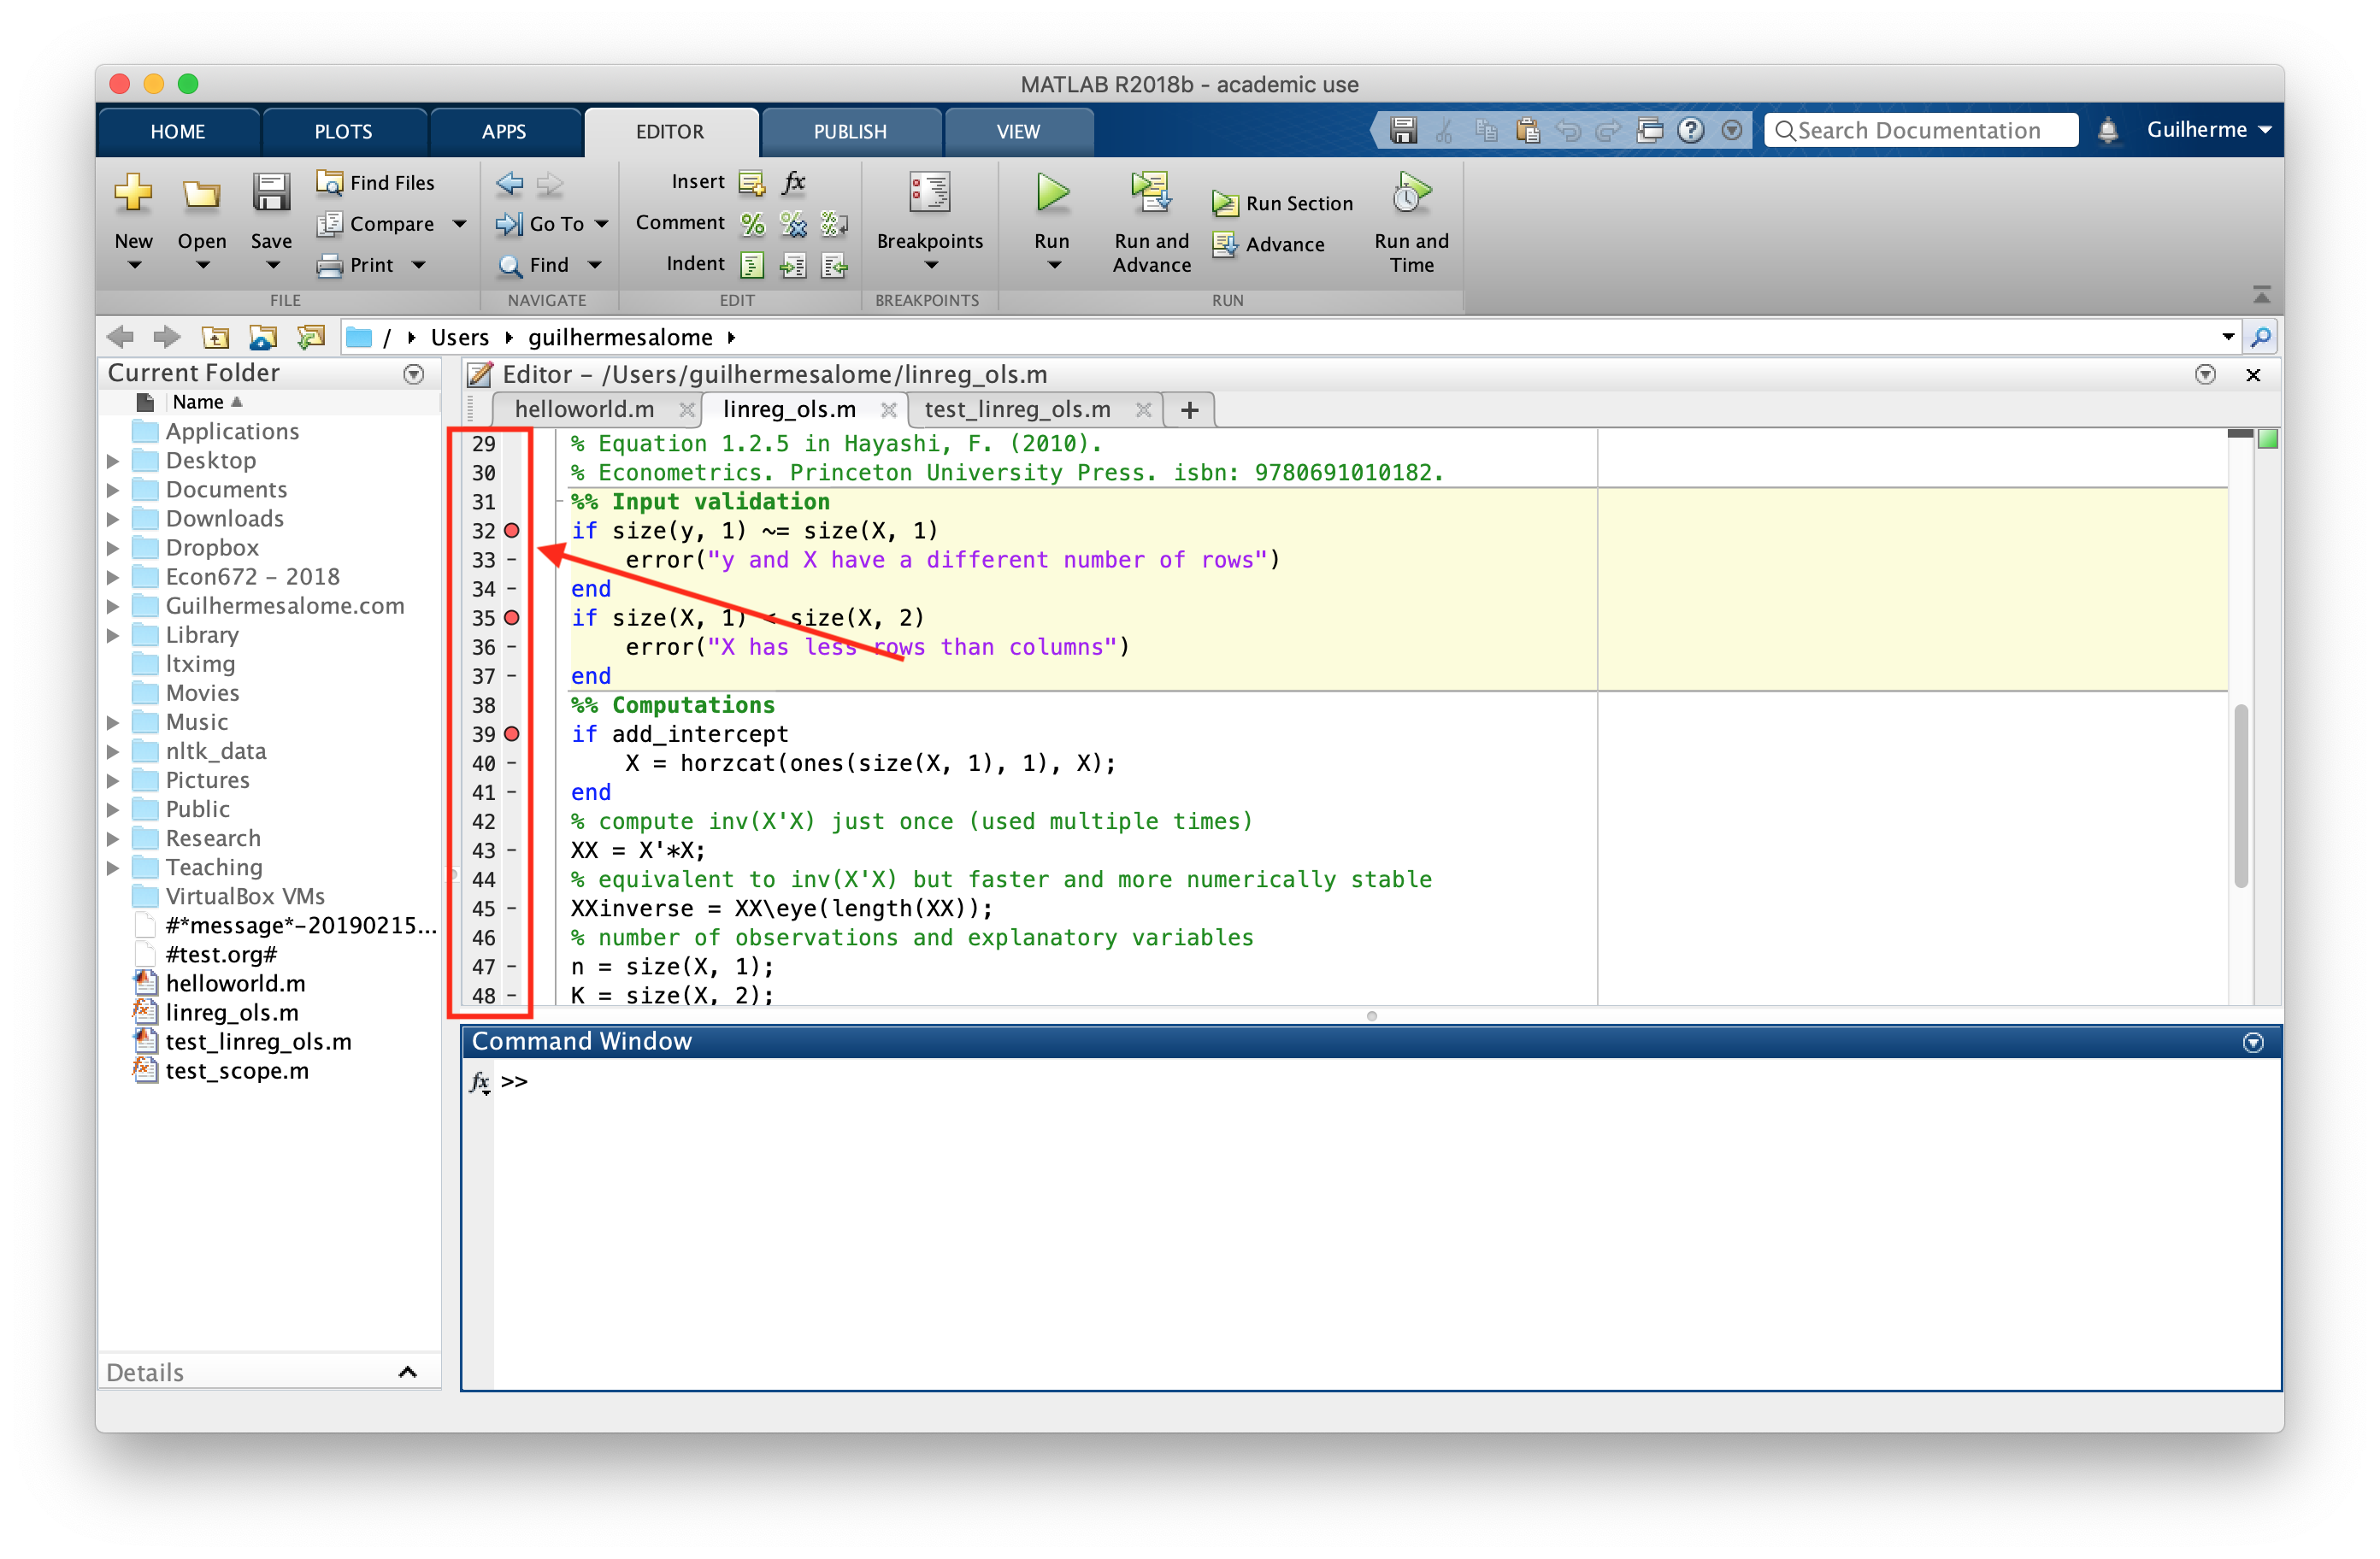
\includegraphics[width=.9\linewidth]{/Users/guilhermesalome/Teaching/Duke/Econ890 Matlab - 2019/supporting/matlab_debugging_breakpoints.png}
\caption{\label{fig:org71a5a7e}
Debugging in Matlab by Adding Breakpoints.}
\end{figure}

Now, in the \texttt{Command Window} execute \texttt{linreg\_ols(y, X)}.
The code will start executing and it will stop at the first breakpoint.
A green arrow will indicate where the execution paused, and at the \texttt{Command Window} you will be able to run any code and inspect the values of the variables.
See Figure \ref{fig:org1f5358c} where the code was paused at the first breakpoint.

\begin{figure}[!ht]
\centering
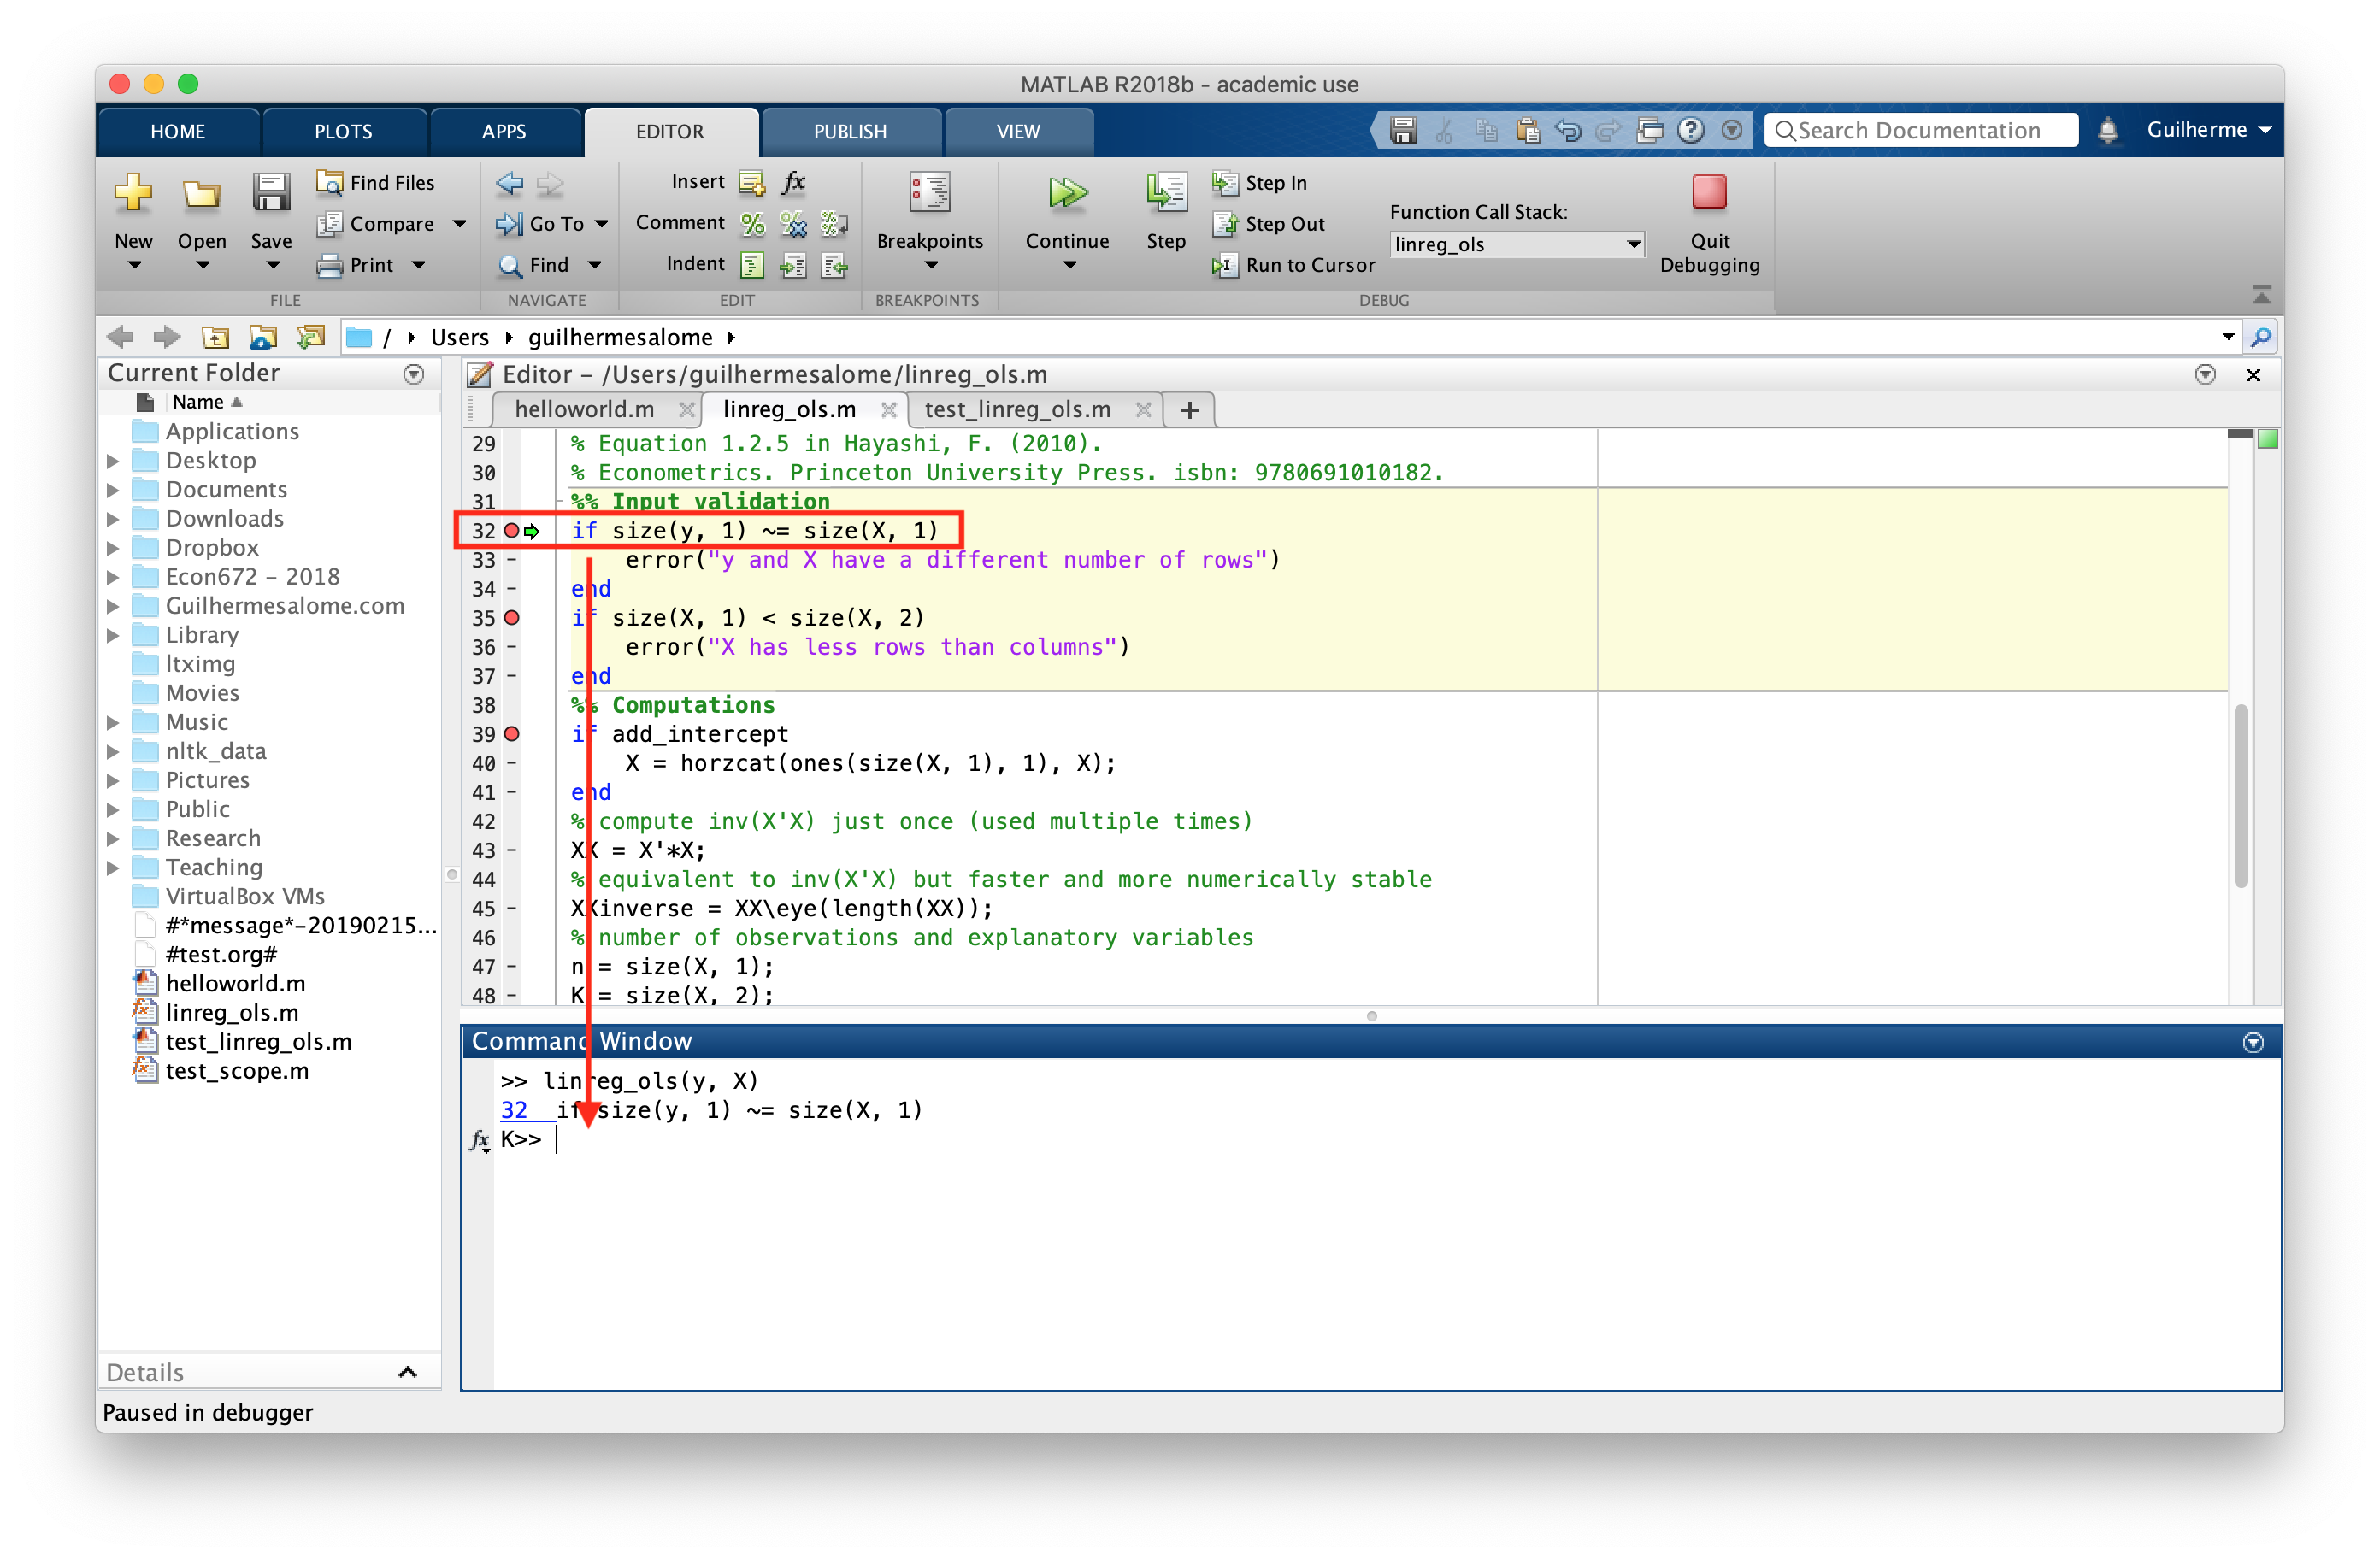
\includegraphics[width=.9\linewidth]{/Users/guilhermesalome/Teaching/Duke/Econ890 Matlab - 2019/supporting/matlab_debugging_paused.png}
\caption{\label{fig:org1f5358c}
Debugging: Execution Paused at Breakpoint.}
\end{figure}

Notice that even though we called \texttt{linreg\_ols} without supplying \texttt{add\_intercept}, the function still executes. You can continue the execution by clicking on the button "Step", see Figure \ref{fig:orga649b58}.

\begin{figure}[!ht]
\centering
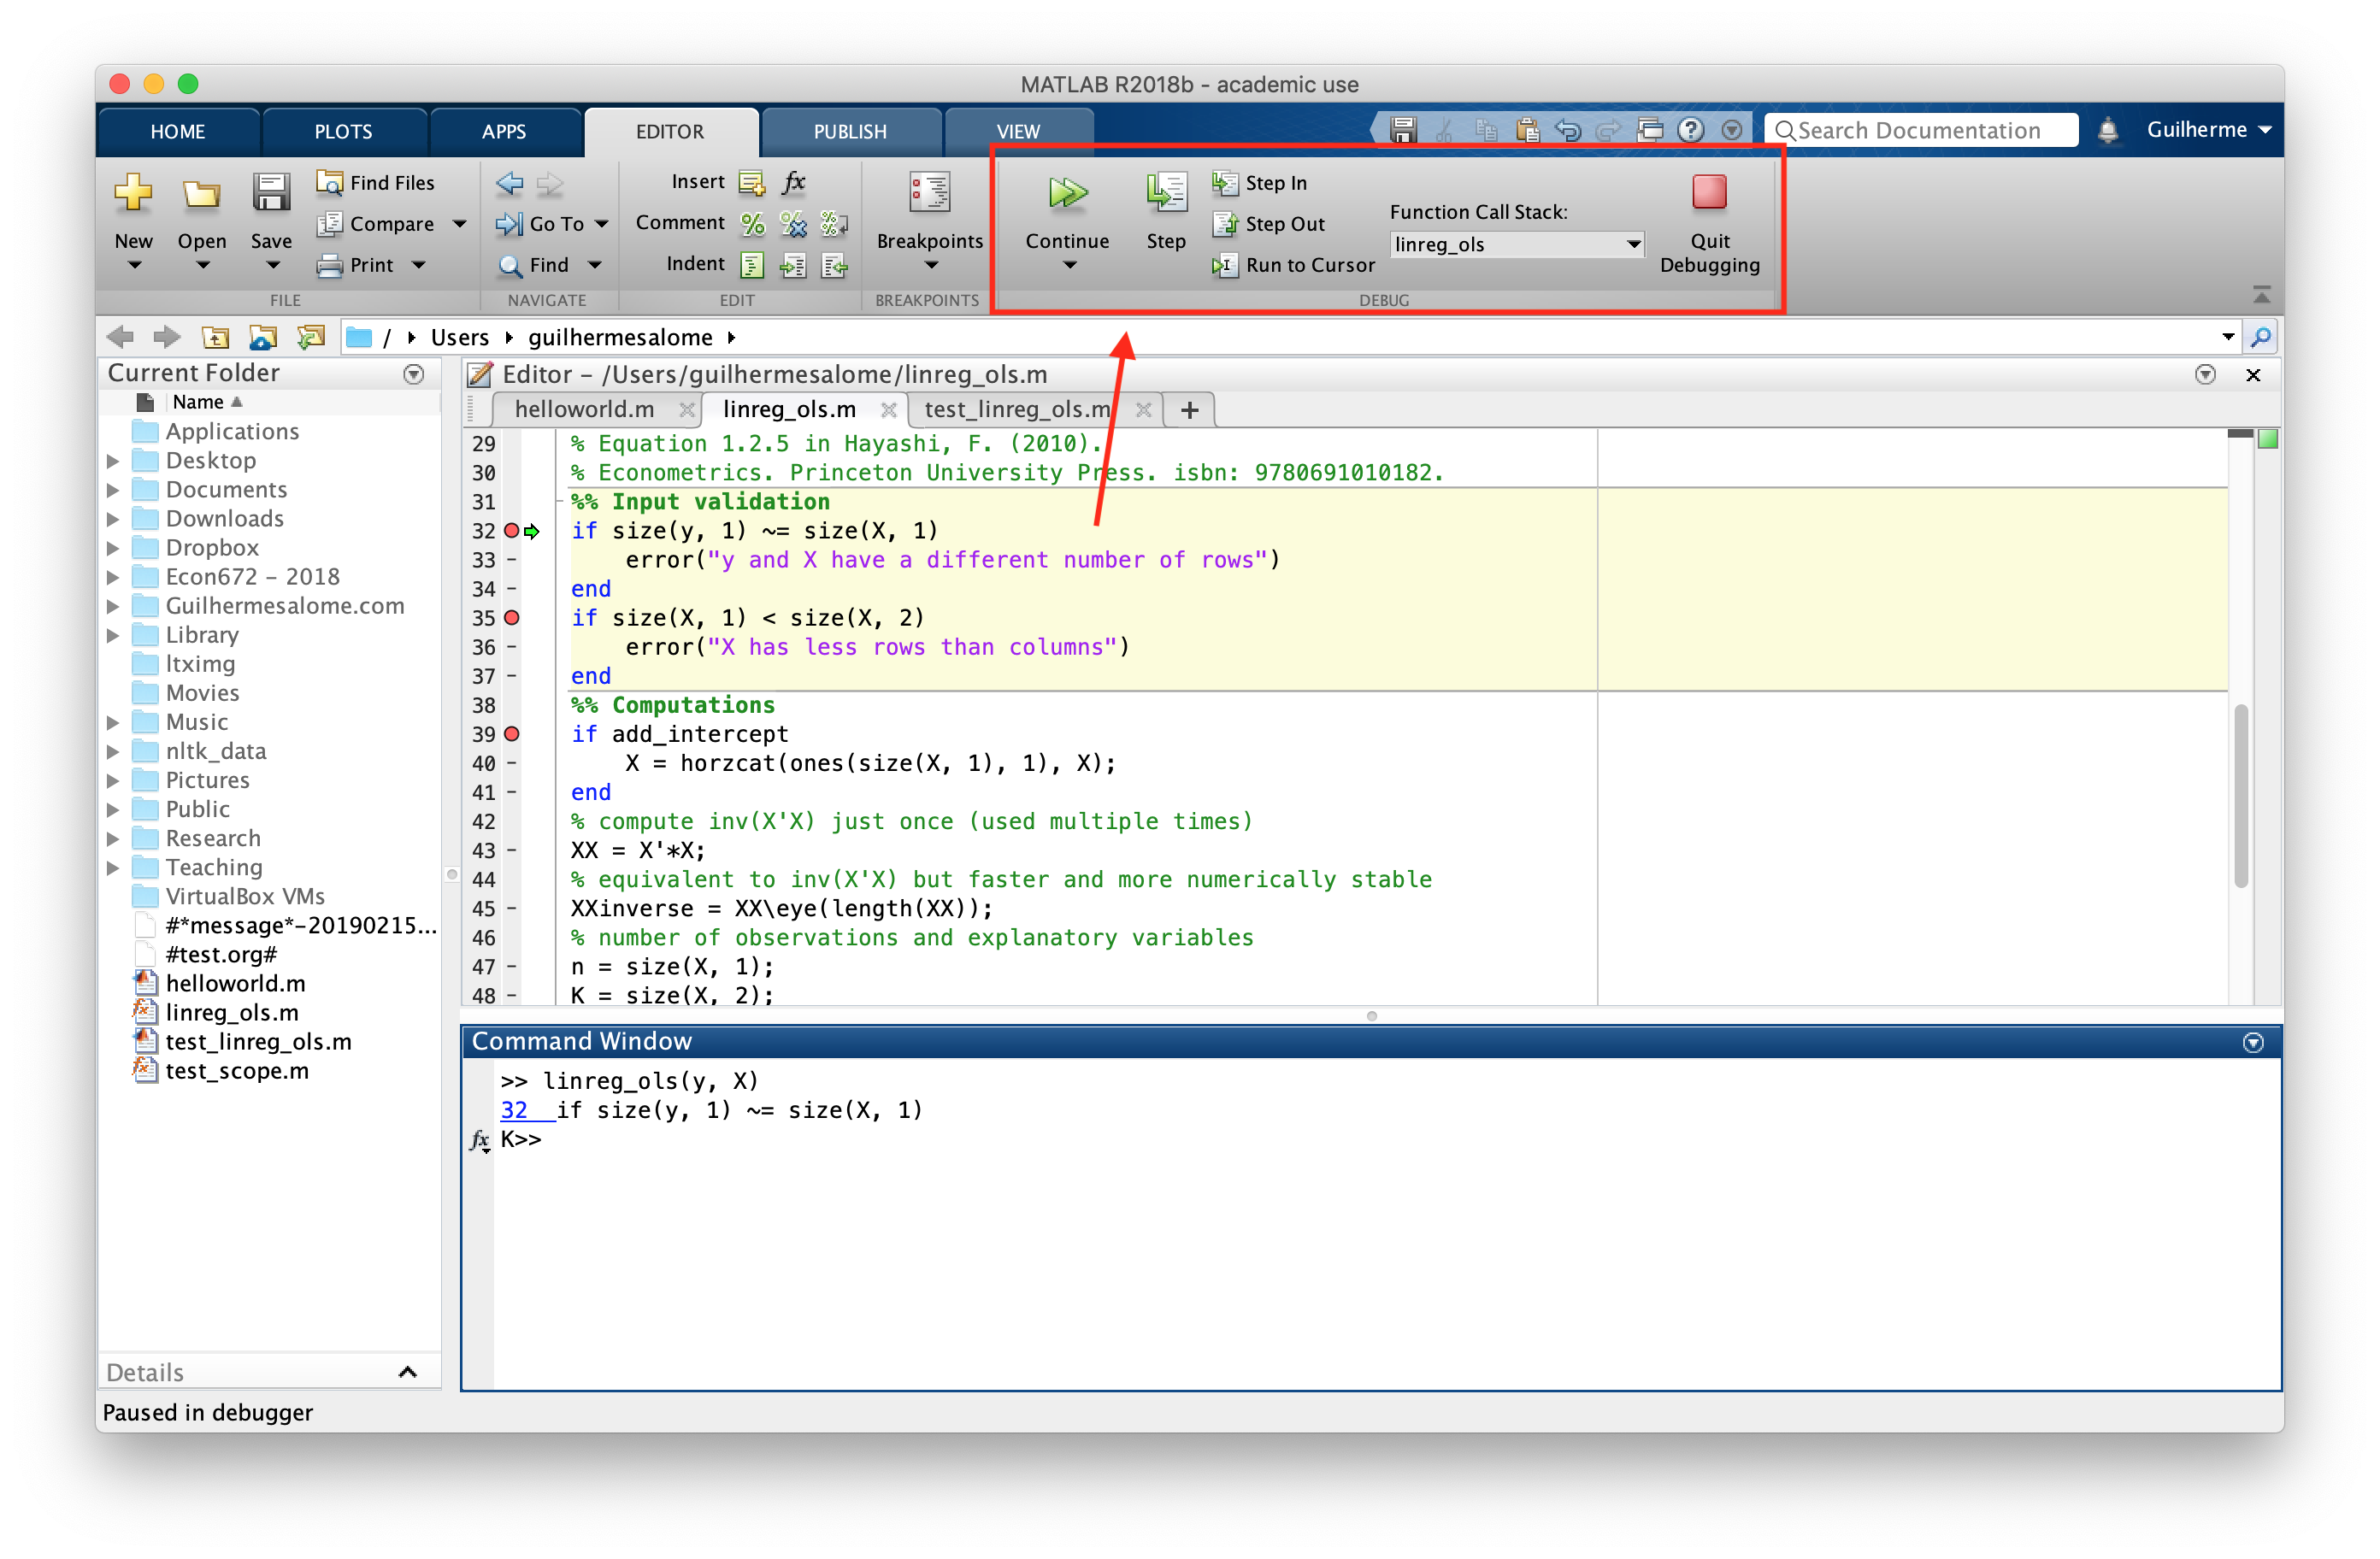
\includegraphics[width=.9\linewidth]{/Users/guilhermesalome/Teaching/Duke/Econ890 Matlab - 2019/supporting/matlab_debugging_continue.png}
\caption{\label{fig:orga649b58}
Debugging: Continue Execution.}
\end{figure}

Keep clicking on "Step" until the code is paused at the third breakpoint.
At this time, the variable \texttt{add\_intercept} is not defined, and if you continue the execution you will get an error message.

Debugging is useful when dealing with large amounts of code and provides a way to ascertain the value of variables in your program.
The code for \texttt{linreg\_ols} will run even if the \texttt{add\_intercept} variable is not passed, but will raise an error as soon as this variable is required.
We can modify our code to allow \texttt{add\_intercept} to be truly an optional variable, so that if it is omitted some default behavior will occur.
\subsection{Optional Variables and Default Values}
\label{sec:org73aac64}
In Matlab, we can add optional variables to a function by passing the keyword \href{https://www.mathworks.com/help/matlab/ref/varargin.html}{\texttt{varargin}} as an input.
Then, inside the function, a variable named \texttt{varargin} is available and contains all optional arguments passed to it.
Since optional arguments could be of any type, \texttt{varargin} must be able to hold different types of data.

In Matlab, a \href{https://www.mathworks.com/help/matlab/ref/cell.html?s\_tid=doc\_ta}{\texttt{cell array}} is a data type that can hold data of various data types, and is the data type used for \texttt{varargin}.
A \texttt{cell array} is similar to a number array and is indexed in the same way, but each element of a \texttt{cell array} is a \texttt{cell}, and a \texttt{cell} can have any data type.
That is, a single \texttt{cell} can hold a number, a character, a string, or even other arrays.
We can create a \texttt{cell array} with braces \texttt{\{ \}}:
\lstset{language=matlab,label= ,caption= ,captionpos=b,firstnumber=1,numbers=left,style=Matlab-editor}
\begin{lstlisting}
% create a cell array
data = {"Parameters", [1, 2, 3]}
% use () to refer to cells, not their contents
data(1, 1)
data(1, 2)
% to access the actual contents of a cell index with {}
data{1, 1}
data{1, 2}
\end{lstlisting}

We can modify \texttt{linreg\_ols} to accept optional arguments using \texttt{varargin}.
Inside \texttt{linreg\_ols}, the variable \texttt{varargin} is a cell array holding any extra inputs passed to the function. If no extra input was passed, then \texttt{varargin} is an empty cell array. We can check whether \texttt{varargin} is empty with the function \texttt{isempty}.
To let the default behavior of the function be adding the intercept, we can verify if \texttt{varargin} is empty, and if it is we add the intercept.
\lstset{language=matlab,label= ,caption= ,captionpos=b,firstnumber=1,numbers=left,style=Matlab-editor}
\begin{lstlisting}
% linreg_ols.m
function results = linreg_ols(y, X, varargin)
%% Input validation
if size(y, 1) ~= size(X, 1)
    error("y and X have a different number of rows")
end
if size(X, 1) < size(X, 2)
    error("X has less rows than columns")
end
%% Add Intercept if Required
if isempty(varargin) || (varargin{1} == true):
    X = horzcat(ones(size(X, 1), 1), X);
end
%% Computations
% compute inv(X'X) just once (used multiple times)
XX = X'*X;
% equivalent to inv(X'X) but faster and more numerically stable
XXinverse = XX\eye(length(XX));
% number of observations and explanatory variables
n = size(X, 1);
K = size(X, 2);
beta = XXinverse*X'*y;
% estimate Var(beta_hat|X)
e = y - X*beta;
s2 = (e'*e)/(n - K);
stderr = diag((s2*XXinverse)^0.5);
% t-statistics
t_stat = beta./stderr;
p_value = (1 - tcdf(abs(t_stat), n - K))*2;
% create results struct
results = struct('b', beta, 's2', s2, 'stderr', stderr, ...
                 't_stat', t_stat, 'p_value', p_value);
end
\end{lstlisting}
It is possible to tie together optional inputs and input validation.
\subsection{Parsing Inputs}
\label{sec:orgff72df4}
Matlab has a built-in way to do input parsing and allowing optional inputs: \href{https://www.mathworks.com/help/matlab/ref/inputparser.html}{\texttt{inputParser}}.
The \texttt{inputParser} is an object created inside a function, which takes care of parsing inputs.

We use the \texttt{inputParser} by first creating a \texttt{parser object}.
Then, we tell this \texttt{parser object} what are the inputs the function should receive.
For example, we tell the \texttt{parser object} it \uline{must} receive a variable named \(y\), it \uline{must} receive a variable named \(X\), and that it \uline{could} receive a variable named \texttt{intercept}.
We can also tell the \texttt{parser object} what conditions each variable must satisfy for it to be accepted and the function to run normally.
We then tell the \texttt{parser object} to parse the inputs, and the parsed inputs will be available in the \texttt{parser object} as a \texttt{struct}.
Let's do an example:
\lstset{language=matlab,label= ,caption= ,captionpos=b,firstnumber=1,numbers=left,style=Matlab-editor}
\begin{lstlisting}
% example_inputparser.m
function example_inputparser(arg1, arg2, varargin)
% create the parser object
parser = inputParser;
% add a required argument to the parser: arg1
addRequired(parser, 'arg1');
% add a required argument to the parser: arg2
addRequired(parser, 'arg2');
% add an optional argument to the parser
addOptional(parser, 'intercept', true);
% actually parse the inputs
parse(parser, arg1, arg2, varargin{:});
inputs = parser.Results;
% display the inputs
disp({inputs.arg1, inputs.arg2, inputs.intercept});
end
\end{lstlisting}
The \texttt{inputParser} code above is quite more extensive than what we had before, but the code itself is also very clear on what it is doing (it is \href{https://en.wikipedia.org/wiki/Self-documenting\_code}{self-documenting}).
We create the \texttt{parser} object, and add two required arguments with the \texttt{addRequired} function.
The \texttt{addRequired} function informs the \texttt{parser} object that it must receive two variables, the first variable should receive the name \texttt{arg1} and the second variable should receive the name \texttt{arg2}.
Then, we call \texttt{addOptional} to inform the \texttt{parser} object that it can receive a third variable, and if it does, this variable should be named \texttt{intercept}.
If no third variable is received, then the variable \texttt{intercept} should be created and its value should be \texttt{true}.
Test the function by calling:
\lstset{language=matlab,label= ,caption= ,captionpos=b,firstnumber=1,numbers=left,style=Matlab-editor}
\begin{lstlisting}
example_inputparser(1, 2)
example_inputparser(1, 2, false)
example_inputparser()
\end{lstlisting}

The functions \texttt{addRequired} and \texttt{addOptional} define inputs that must appear in the correct order (positional arguments). While \texttt{addRequired} defines required inputs, \texttt{addOptional} defines optional inputs, but both inputs are positional arguments.
However, we can also define inputs that can come in different order, but to do so these inputs must also be named (name-value pair arguments).
We can add these name-value pair inputs with the \texttt{addParameter} function:
\lstset{language=matlab,label= ,caption= ,captionpos=b,firstnumber=1,numbers=left,style=Matlab-editor}
\begin{lstlisting}
% example_inputparser.m
function example_inputparser(arg1, arg2, varargin)
% create the parser object
parser = inputParser;
% add a required argument to the parser: arg1
addRequired(parser, 'arg1');
% add a required argument to the parser: arg2
addRequired(parser, 'arg2');
% add an optional argument to the parser
addOptional(parser, 'intercept', true);
% add a name-value pair input to the parser
addParameter(parser, 'cov_type', 'standard');
% actually parse the inputs
parse(parser, arg1, arg2, varargin{:});
inputs = parser.Results;
% display the inputs
disp({inputs.arg1, inputs.arg2, inputs.intercept, inputs.cov_type});
end
\end{lstlisting}
The order for inputs is always the following: required arguments, optional arguments, name-value pairs.

The advantage of using \texttt{inputParser} is that we can also do input validation at the same time. Each of the functions \texttt{addRequired}, \texttt{addOptional} and \texttt{addParameter} can take a validation function that is used to check whether the inputs are valid.
Let's add input validation to \texttt{example\_inputparser}:
\lstset{language=matlab,label= ,caption= ,captionpos=b,firstnumber=1,numbers=left,style=Matlab-editor}
\begin{lstlisting}
% example_inputparser.m
function example_inputparser(arg1, arg2, varargin)
% create the parser object
parser = inputParser;
% add a required argument to the parser: arg1
addRequired(parser, 'arg1', @validate_arg1);
% add a required argument to the parser: arg2
addRequired(parser, 'arg2', @validate_arg2);
% add an optional argument to the parser
addOptional(parser, 'intercept', true, @validate_intercept);
% add a name-value pair input to the parser
addParameter(parser, 'cov_type', 'standard', @validate_cov_type);
% actually parse the inputs
parse(parser, arg1, arg2, varargin{:});
inputs = parser.Results;
% display the inputs
disp({inputs.arg1, inputs.arg2, inputs.intercept, inputs.cov_type});
end

%% Functions for input validation
% these functions must return a boolean value or throw an error
function bool = validate_arg1(arg1)
    bool = isnumeric(arg1);
end

function bool = validate_arg2(arg2)
    bool = isnumeric(arg2) && size(arg2, 1) >= size(arg2, 2);
end

function bool = validate_intercept(intercept)
    bool = islogical(intercept) && length(intercept) == 1;
end

function bool = validate_cov_type(cov_type)
    covs = ["standard", "White", "HAC"];
    bool = ischar(cov_type) && ismember(cov_type, covs);
end
\end{lstlisting}
The functions declared in the section "Functions for input validation" are passed as arguments to the functions \texttt{addRequired}, \texttt{addOptional} and \texttt{addParameter}.
To pass a function as an argument to another function we use the \texttt{@} operator in front of the function name.
When we use the \texttt{@} syntax with the function name we are creating a \href{https://www.mathworks.com/help/matlab/matlab\_prog/creating-a-function-handle.html}{function handle}.
A function handle allows a function to be passed around as any other variable, and calling a function handle is the same as calling the function itself.

Notice that most of the functions above have just one line of code.
We can simplify the code by using anonymous functions.
\subsection{Anonymous Functions}
\label{sec:org7424a5b}
An \href{https://www.mathworks.com/help/matlab/matlab\_prog/anonymous-functions.html}{anonymous function} is a function that is written in a single line and is itself a function handle.
We can create an anonymous function using the syntax \texttt{@(inputs) code;}.
For example:
\lstset{language=matlab,label= ,caption= ,captionpos=b,firstnumber=1,numbers=left,style=Matlab-editor}
\begin{lstlisting}
% create an anonymous function and assign to a variable
square_root = @(x) x.^0.5;
% call the anonymous function
square_root(4)
% since the anonymous function is a function handle
% we can pass it as inputs to other functions
integral(square_root, 0, 1)
% we can create an anonymous within an anonymous function
poly_integral = @(a) integral(@(x) (a*x.^2 + x + 2), 0, 1);
\end{lstlisting}

The validating functions in \texttt{example\_inputparser} can be substituted by anonymous functions, which makes the code clearer.
Let's modify \texttt{example\_inputparser} to make use of anonymous functions:
\lstset{language=matlab,label= ,caption= ,captionpos=b,firstnumber=1,numbers=left,style=Matlab-editor}
\begin{lstlisting}
% example_inputparser.m
function example_inputparser(arg1, arg2, varargin)
% create the parser object
parser = inputParser;
% add a required argument to the parser: arg1
addRequired(parser, 'arg1', @isnumeric);
% add a required argument to the parser: arg2
addRequired(parser, 'arg2', @(x) (isnumeric(x) && size(x, 1) >= size(x, 2)));
% add an optional argument to the parser
addOptional(parser, 'intercept', true, @(x) (islogical(x) && length(x) == 1));
% add a name-value pair input to the parser
addParameter(parser, 'cov_type', 'standard', @validate_cov_type);
% actually parse the inputs
parse(parser, arg1, arg2, varargin{:});
inputs = parser.Results;
% display the inputs
disp({inputs.arg1, inputs.arg2, inputs.intercept, inputs.cov_type});
end

%% Functions for input validation
% these functions must return a boolean value or throw an error
function bool = validate_cov_type(cov_type)
    covs = ["standard", "White", "HAC"];
    bool = ischar(cov_type) && ismember(cov_type, covs);
end
\end{lstlisting}

We can make use of these features to validate the input for \texttt{linreg\_ols}:
\lstset{language=matlab,label= ,caption= ,captionpos=b,firstnumber=1,numbers=left,style=Matlab-editor}
\begin{lstlisting}
% linreg_ols.m
function results = linreg_ols(y, X, varargin)
%% Input validation
parser = inputParser;
addRequired(parser, 'y', @isnumeric)
addRequired(parser, 'X', @validate_X);
addParameter(parser, 'intercept', true, @islogical);
parse(parser, y, X, varargin{:});
y = parser.Results.y;
X = parser.Results.X;
if size(y, 1) ~= size(X, 1)
    error("y and X have a different number of rows")
end
%% Add Intercept if Required
if parser.Results.intercept
    X = horzcat(ones(size(X, 1), 1), X);
end
%% Computations
% compute inv(X'X) just once (used multiple times)
XX = X'*X;
% equivalent to inv(X'X) but faster and more numerically stable
XXinverse = XX\eye(length(XX));
% number of observations and explanatory variables
n = size(X, 1);
K = size(X, 2);
beta = XXinverse*X'*y;
% estimate Var(beta_hat|X)
e = y - X*beta;
s2 = (e'*e)/(n - K);
stderr = diag((s2*XXinverse)^0.5);
% t-statistics
t_stat = beta./stderr;
p_value = (1 - tcdf(abs(t_stat), n - K))*2;
% create results struct
results = struct('b', beta, 's2', s2, 'stderr', stderr, ...
                 't_stat', t_stat, 'p_value', p_value);
end

%% Functions for Input Validation
function bool = validate_X(X)
    bool = isnumeric(X);
    if size(X, 1) < size(X, 2)
        error("X has less rows than columns");
    end
end
\end{lstlisting}
We can now call \texttt{linreg\_ols} with or without a name-value pair specifying the inclusion of an intercept:
\lstset{language=matlab,label= ,caption= ,captionpos=b,firstnumber=1,numbers=left,style=Matlab-editor}
\begin{lstlisting}
linreg_ols(y, X)
linreg_ols(y, X, 'intercept', true)
\end{lstlisting}
\section{Importing Data and Saving Results}
\label{sec:org2520fd5}
We will now use our \texttt{linreg\_ols} function with a real data set.
Download \href{https://raw.githubusercontent.com/Salompas/handson-ml/master/datasets/housing/housing.csv}{this data set on housing prices in California}, and save the file in your working folder.
This data set was first used in \citet{PB1997}, and was later modified for use in \citet{G2017}.
The data contains information on household prices in California in 1990 (based on the census at that time).
The first line of the file contains the name of the explanatory variables.
\subsection{Importing Data}
\label{sec:orgab1b423}
Matlab has various built-in functions for \href{https://www.mathworks.com/help/matlab/data-import-and-export.html}{importing data of different types}.
We can import \texttt{.csv} files to Matlab with the \href{https://www.mathworks.com/help/matlab/ref/readmatrix.html}{\texttt{readmatrix}} function\footnote{There is also a GUI interface for importing data under the menu tab \texttt{Home}, via the button \texttt{Import Data}. Older versions of Matlab have different functions for importing data. Before the R2019a release, for example, \texttt{.csv} files could be imported with the function \texttt{csvread}. You can still use \texttt{csvread}, but \texttt{readmatrix} should be preferred since it is an improved version.}.
\lstset{language=matlab,label= ,caption= ,captionpos=b,firstnumber=1,numbers=left,style=Matlab-editor}
\begin{lstlisting}
data = readmatrix('housing.csv');
\end{lstlisting}
The default behavior of \texttt{readmatrix} is to infer the type of the file from its extension, in this case \texttt{.csv}.
Knowing the file extension, the function knows that the values are comma-separated, and the function also attempts to detect if there is a header line and the number of variables (columns) to be imported.
The \texttt{housing.csv} data is mostly numeric, with the exception of the last column.
The function \texttt{readmatrix} imports the data into a numeric matrix, which works well for the first 9 columns of \texttt{housing.csv}.
However, the last column of the file contains categorical data, which is not automatically converted to numbers, and so Matlab treats all its values as \texttt{NaN}.
If we are not interested in using the last column we could work with \texttt{readmatrix}.

The resulting \texttt{data} matrix has all the information from \texttt{housing.csv}, with the exception of the names of the variables and the last column of the file.
We can keep all the columns of the data and the names of the variables if we import the data to a \texttt{table} instead of a numeric array.
To do so, we use the function \href{https://www.mathworks.com/help/matlab/ref/readtable.html}{\texttt{readtable}}.
As with \texttt{readmatrix}, the function \texttt{readtable} can figure out the delimiter, header and number of variables from the file extension, but instead of loading the data into a numeric array, it loads the data into a \href{https://www.mathworks.com/help/matlab/ref/table.html}{\texttt{table}}.
\lstset{language=matlab,label= ,caption= ,captionpos=b,firstnumber=1,numbers=left,style=Matlab-editor}
\begin{lstlisting}
% import housing data
data = readtable('housing.csv');
% verify that everything was imported correctly
data(1:5, :)
% notice that the names of the variables are also
% displayed, and that the last is correctly imported

% data in a table can be accessed by normal indexing as in a
% numeric array
data(1:10, 1)
data(1:10, 2)
data(1:10, 10)
% but we can also access the data like in a struct, where the field
% names are the variable names
data.longitude
data.longitude(1:5)
data.ocean_proximity(1:5)
% notice that the ocean_proximity data is stored as character
% arrays in cells
% we can convert it to a string array:
data.ocean_proximity = string(data.ocean_proximity);
data.ocean_proximity(1:10)
% we can see all the variable names in a table via its properties
data.Properties.VariableNames
% we can access the columns of the table by index with the names
data(1:5, 'longitude')
% for multiple columns we pass a string array
data(1:5, ["population", "households", "median_income"])
% similar to cells, when we index with parentheses we do not get the
% actual values stored in a table, but we get a subtable
% to get the actual values we use the curly brackets notation
data{1:5, ["population", "households", "median_income"]}
\end{lstlisting}

The data has a few missing values (added on purpose).
We can count how many lines have missing values with the functions \texttt{isnan} and \texttt{sum}.
The function \texttt{isnan} takes a numeric array and finds all \texttt{NaN}.
The function \texttt{sum} can be used to sum across values in rows or columns (or both) of a matrix.
\lstset{language=matlab,label= ,caption= ,captionpos=b,firstnumber=1,numbers=left,style=Matlab-editor}
\begin{lstlisting}
% dimensions of table
size(data)
% find missing data no the first column
sum(isnan(data{:, 1}))
% find missing data on all columns, except the last one
sum(isnan(data{:, 1:9}))
% we see that there are 207 missing data points for the
% total_bedrooms variable
% indeed:
sum(isnan(data.total_bedrooms))
% let's remove these rows from the table
% first we need to find the indices for the rows with missing values
missing_values = isnan(data.total_bedrooms);
% missing_values is a boolean array, it has 1's where there are
% NaNs in the data.total_bedrooms array
% we can use this logical (boolean) array to index the original
% table and select only the rows without NaN's
data_no_missing = data(~missing_values, :);
% this gives us a new table, from which we can extract data for the regression
\end{lstlisting}

We can also remove rows with missing values (represented by \texttt{NaN}) automatically using the function \href{https://www.mathworks.com/help/matlab/ref/rmmissing.html}{\texttt{rmmissing}}:
\lstset{language=matlab,label= ,caption= ,captionpos=b,firstnumber=1,numbers=left,style=Matlab-editor}
\begin{lstlisting}
size(data)
data_no_missing = rmmissing(data);
size(data_no_missing)
\end{lstlisting}

Let's run a regression of the logarithm of the median house value on the logarithm of the number of bedrooms in the house.
\lstset{language=matlab,label= ,caption= ,captionpos=b,firstnumber=1,numbers=left,style=Matlab-editor}
\begin{lstlisting}
results = linreg_ols(log(data.median_house_value), ...
                     log(data.total_bedrooms));
disp(results.b);
\end{lstlisting}
\subsection{Saving Results, Cleaning the Workspace and Loading Variables}
\label{sec:org689afac}
Now that we can generate results from data, we need to save these results.
\href{https://www.mathworks.com/help/matlab/matlab\_env/save-load-and-delete-workspace-variables.html}{Saving and loading variables in Matlab} can be done with the functions \href{https://www.mathworks.com/help/matlab/ref/save.html}{\texttt{save}} and \href{https://www.mathworks.com/help/matlab/ref/load.html}{\texttt{load}}.
There are several ways of using the function \texttt{save}:
\lstset{language=matlab,label= ,caption= ,captionpos=b,firstnumber=1,numbers=left,style=Matlab-editor}
\begin{lstlisting}
% Save ALL variables in the workspace
save('all_workspace_variables');
% The above creates a file named all_workspace_variables.mat
% .mat files can be easily imported with the load function

% Save only ONE variable
save('housing_clean', 'data_no_missing');
% saves the variable data_no_missing on the file housing_clean.mat

% Save MULTIPLE variables
save('data_and_results', 'data_no_missing', 'results');
% saves the variables data_no_missing and results in
% the file data_and_results.mat
\end{lstlisting}
The files created with the function \texttt{save} have the \texttt{.mat} extension and are binary files.

Let's now clear our workspace to and reload the variables.
First, clear the command window by executing \href{https://www.mathworks.com/help/matlab/ref/clc.html}{\texttt{clc}}.
This command simply clears the \texttt{Command Window} so that you have a clear screen to type commands.
You can still use the arrow keys to execute previous commands.
Second, use the special command \href{https://www.mathworks.com/help/matlab/ref/clear.html}{\texttt{clear}} to delete all variables from the workspace.
After executing this command the variables previously created are gone.
It is also possible to clear specific variables by executing \texttt{clear variable\_name}.
Third, use \texttt{load} to load the \texttt{.mat} files, which will take the variables stored in those files and make them available in the workspace.
\lstset{language=matlab,label= ,caption= ,captionpos=b,firstnumber=1,numbers=left,style=Matlab-editor}
\begin{lstlisting}
% Load ALL variables from before
load('all_workspace_variables.mat');
% Load only the HOUSING variable from before
clear;
load('all_workspace_variables.mat', 'housing');
% Notice we pass the name of the variable to load so that only that
% variable is loaded
% Load the cleaned housing data
clear;
load('housing_clean.mat');
% Load the cleaned housing data and the regression results
clear;
load('data_and_results.mat');
% Load only the regression results
clear;
load('data_and_results.mat', 'results');
\end{lstlisting}
Notice that the variables are loaded with their original names.
\section{Summary}
\label{sec:org6c006f9}
We have covered the basics of the Matlab programming language.
You should be able to:
\begin{itemize}
\item Create \texttt{.m} script files to run code
\item Work with vectors and matrices
\item Do basic computations and linear algebra with numeric arrays
\item Create function files
\item Use conditionals
\item Use for-loops and while-loops
\item Generate data from statistical distributions
\item Create arrays for text data
\item Present data in a neat manner using \texttt{table}
\item Organize function results in \texttt{struct}
\item Validate input variables with conditionals
\item Debug code with the built-in debugger
\item Let functions accept any number of inputs with \texttt{varargin}
\item Use \texttt{inputParser} to parse input variables and specify default values
\item Pass functions as arguments with function handles
\item Simplify small functions with anonymous functions
\item Import \texttt{.csv} data
\item Clean rows from a table with missing values
\item Save variables to \texttt{.mat} files
\item Clear the workspace
\item Load variables stored in \texttt{.mat} files
\end{itemize}
\section{Assignment}
\label{sec:org2f29049}
All assignments should be submitted to the Github repository you have been assigned to.
The deadline is July 26th by midnight.
You should write a report in Latex with the solutions to the problems below.
If the problem requires you to code, then the code should also be included in the report.
For a quick guide on how to add Matlab code to your Latex files, refer to the Section "Adding Matlab Code" on \href{https://guilhermesalome.com/teaching/2018-empirical-methods-in-financial-econometrics/posts/lecture-1-latex.html\#org61c35bc}{this tutorial}.

\begin{problem}
Update the code for generating data to function without loops (vectorization).
To do so, you will need to read the documentation for the random number generator functions we have used: \href{https://www.mathworks.com/help/matlab/ref/rand.html}{\texttt{rand}} and \href{https://www.mathworks.com/help/matlab/ref/randn.html}{\texttt{randn}}.
After vectorizing the problem, verify you get the same estimates for the parameters as before.
For this part, you will need to fix the generation of random numbers, so that you generate the same random numbers when you run your code without vectorization and with vectorization.
Read the \href{https://www.mathworks.com/help/matlab/ref/rng.html}{documentation} for the \texttt{rng} function, and if you need more details read about \href{https://www.mathworks.com/help/matlab/math/managing-the-global-stream.html}{managing the global stream}.
\end{problem}

\begin{problem}
Extend \texttt{linreg\_ols} to also output the \(R^2\) of the regression (see Equation 1.2.18 in \citet{H2000}.
\end{problem}

\begin{problem}
Run the linear regression suggested in Equation (8) of \citet{PB1997}.
\end{problem}

\begin{problem}
Matlab has been around \href{https://www.mathworks.com/company/newsletters/articles/a-brief-history-of-matlab.html}{since 1984} and has many packages for common problems.
Figure out if Matlab has a function for estimating the parameters of a linear regression using OLS.
If it does, what is the name of the function?
How does the function actually estimate the coefficients?
To answer this, you need to look at the code of the function.
You can do so with the special command \href{https://www.mathworks.com/help/matlab/ref/type.html}{\texttt{type}}.
For example, if the name of the function is \texttt{ols}, then you can execute \texttt{type ols} to see the source code.
\end{problem}

\begin{problem}
When the classical assumption of homoskedasticity fails, we need a different estimators for the standard errors of the OLS estimates.
\citet{W1980} proposes a heteroskedasticity-robust estimator for the standard errors of the OLS estimates, which is now known as White's standard error.
Equation 2.4.1 in \citet{H2000} shows White's standard error:
\begin{align*}
\widehat{SE(\hat{\beta}_i)}\equiv\sqrt{\frac{1}{n}[S_{xx}^{-1}\hat{S}S_{xx}^{-1}]_{[i,i]}}
\end{align*}
There is a slight change of notation in this part of the \citet{H2000}, and \(x_i'\) is the ith row of \(X\) (\(x_i\) is a column vector with the explanatory variables in the ith row of \(X\)).
The term \(S_{xx}\) is the sample mean of \(x_ix_i'\): \(S_{xx}=\frac{1}{n}\sum_{i=1}^nx_ix_i'\) (Equation 2.3.6 in \citet{H2000}).
The term \(\hat{S}\) is an estimator for a matrix of fourth moments, and it is defined as \(\hat{S}=\frac{1}{n}\sum_{i=1}^ne_i^2x_ix_i'\) (Equation 2.5.1 in \citet{H2000}), and \(e_i\) is as before (residual for the ith observation).
Implement this estimator in the \texttt{linreg\_ols} function.
You could write a local function to estimate White's standard error in the \texttt{linreg\_ols.m} file.
\end{problem}

\begin{problem}
(Optional) Implement the t-test based on White's standard error. Also, compute the p-value from given the statistic.
\end{problem}

\begin{problem}
\citet{NW1987} proposes another estimator to the standard errors for the OLS estimates under weaker assumptions.
The estimator the authors propose is robust not only to heteroskedasticity, but also autocorrelation, and is known as the HAC standard errors.
Does Matlab have a function to compute the HAC standard errors?
If so, extend \texttt{linreg\_ols} to also compute the HAC standard errors.
\end{problem}

\begin{problem}
(Optional) Implement the t-test based on the HAC standard error. Also, compute the p-value from given the statistic.
\end{problem}

\begin{problem}
Extend \texttt{linreg\_ols} to accept an optional input named \texttt{cov\_type}, which specifies the type of standard errors estimator to report.
Use \texttt{inputParser} to do so.
\end{problem}
\newpage
\printbibliography
\newpage
\end{document}